% % % % % % % If you have a single appendix, you should be using OneSingleAppendix.tex
% % % % % % % NOT this file

\chapter{EVENT DISPLAYS}

Collision events recorded by the CMS detector can be visualized as event displays using the Fireworks application developed by the CMS collaboration.\cite{Fireworks} Event displays are used to visually summarize particle interactions with the detector's subsystems by rendering reconstructed objects of interest such as particle tracks and jets over a 3D model of the detector. Figures \ref{fig:evt_disp_Znn} through \ref{fig:evt_disp_Zmm} each show multiple different perspectives of an event display for a candidate signal region event from each decay channel. The candidate events were chosen based on their high DNN scores, which indicate that the DNN of their corresponding decay channel classified them as a signal event with high confidence. Although the event metadata are provided on the event displays, other event-level quantities of interest are shown in Table \ref{tbl:event_display}.

\begin{table}[htbp]
  \caption[Event Display Candidate Information]{Information for the candidate signal region events visualized by the event display. The values of the kinematic quantities are reported in units of \GeV\ and the \btag\ algorithm is DeepCSV.}
  \label{tbl:event_display}
  \begin{tabularx}{6.5in}{XXXrrXXXX}
    \hline
    Channel & \mjj   & \pTjj  & \pTjmax & \pTjmin & \btagmax & \btagmin & \pTV   & DNN score \\
    \hline
    \ZnnH   & 121.56 & 319.43 & 195.99  & 129.81  & 0.999    & 0.993    & 319.10 & 0.975     \\
    \WenH   & 126.49 & 259.66 & 179.31  & 87.31   & 0.999    & 0.995    & 295.75 & 0.989     \\
    \WmnH   & 117.69 & 250.55 & 177.33  & 85.28   & 0.996    & 0.995    & 259.80 & 0.993     \\
    \ZeeH   & 114.14 & 286.17 & 216.54  & 97.82   & 0.990    & 0.957    & 311.33 & 1.00      \\
    \ZmmH   & 111.39 & 100.12 & 78.66   & 69.53   & 0.984    & 0.975    & 466.83 & 1.00      \\
    \hline
  \end{tabularx}
\end{table}

For each figure, the perspective of the largest subfigure is a projection of the event display onto the \textit{xz}-plane, unless otherwise specified. The perspective of both of the smaller subfigures is a projection of the event display onto the \textit{xy}-plane, with the subfigure on the right zoomed in on the interaction point. This level of zoom is necessary to show the secondary vertices and their associated tracks, shown in black, and to appreciate that those tracks do not extrapolate well to any of the primary vertices, shown in yellow.

\begin{figure}[htbp]
  \centering
  \mbox{
    \subfigure [] {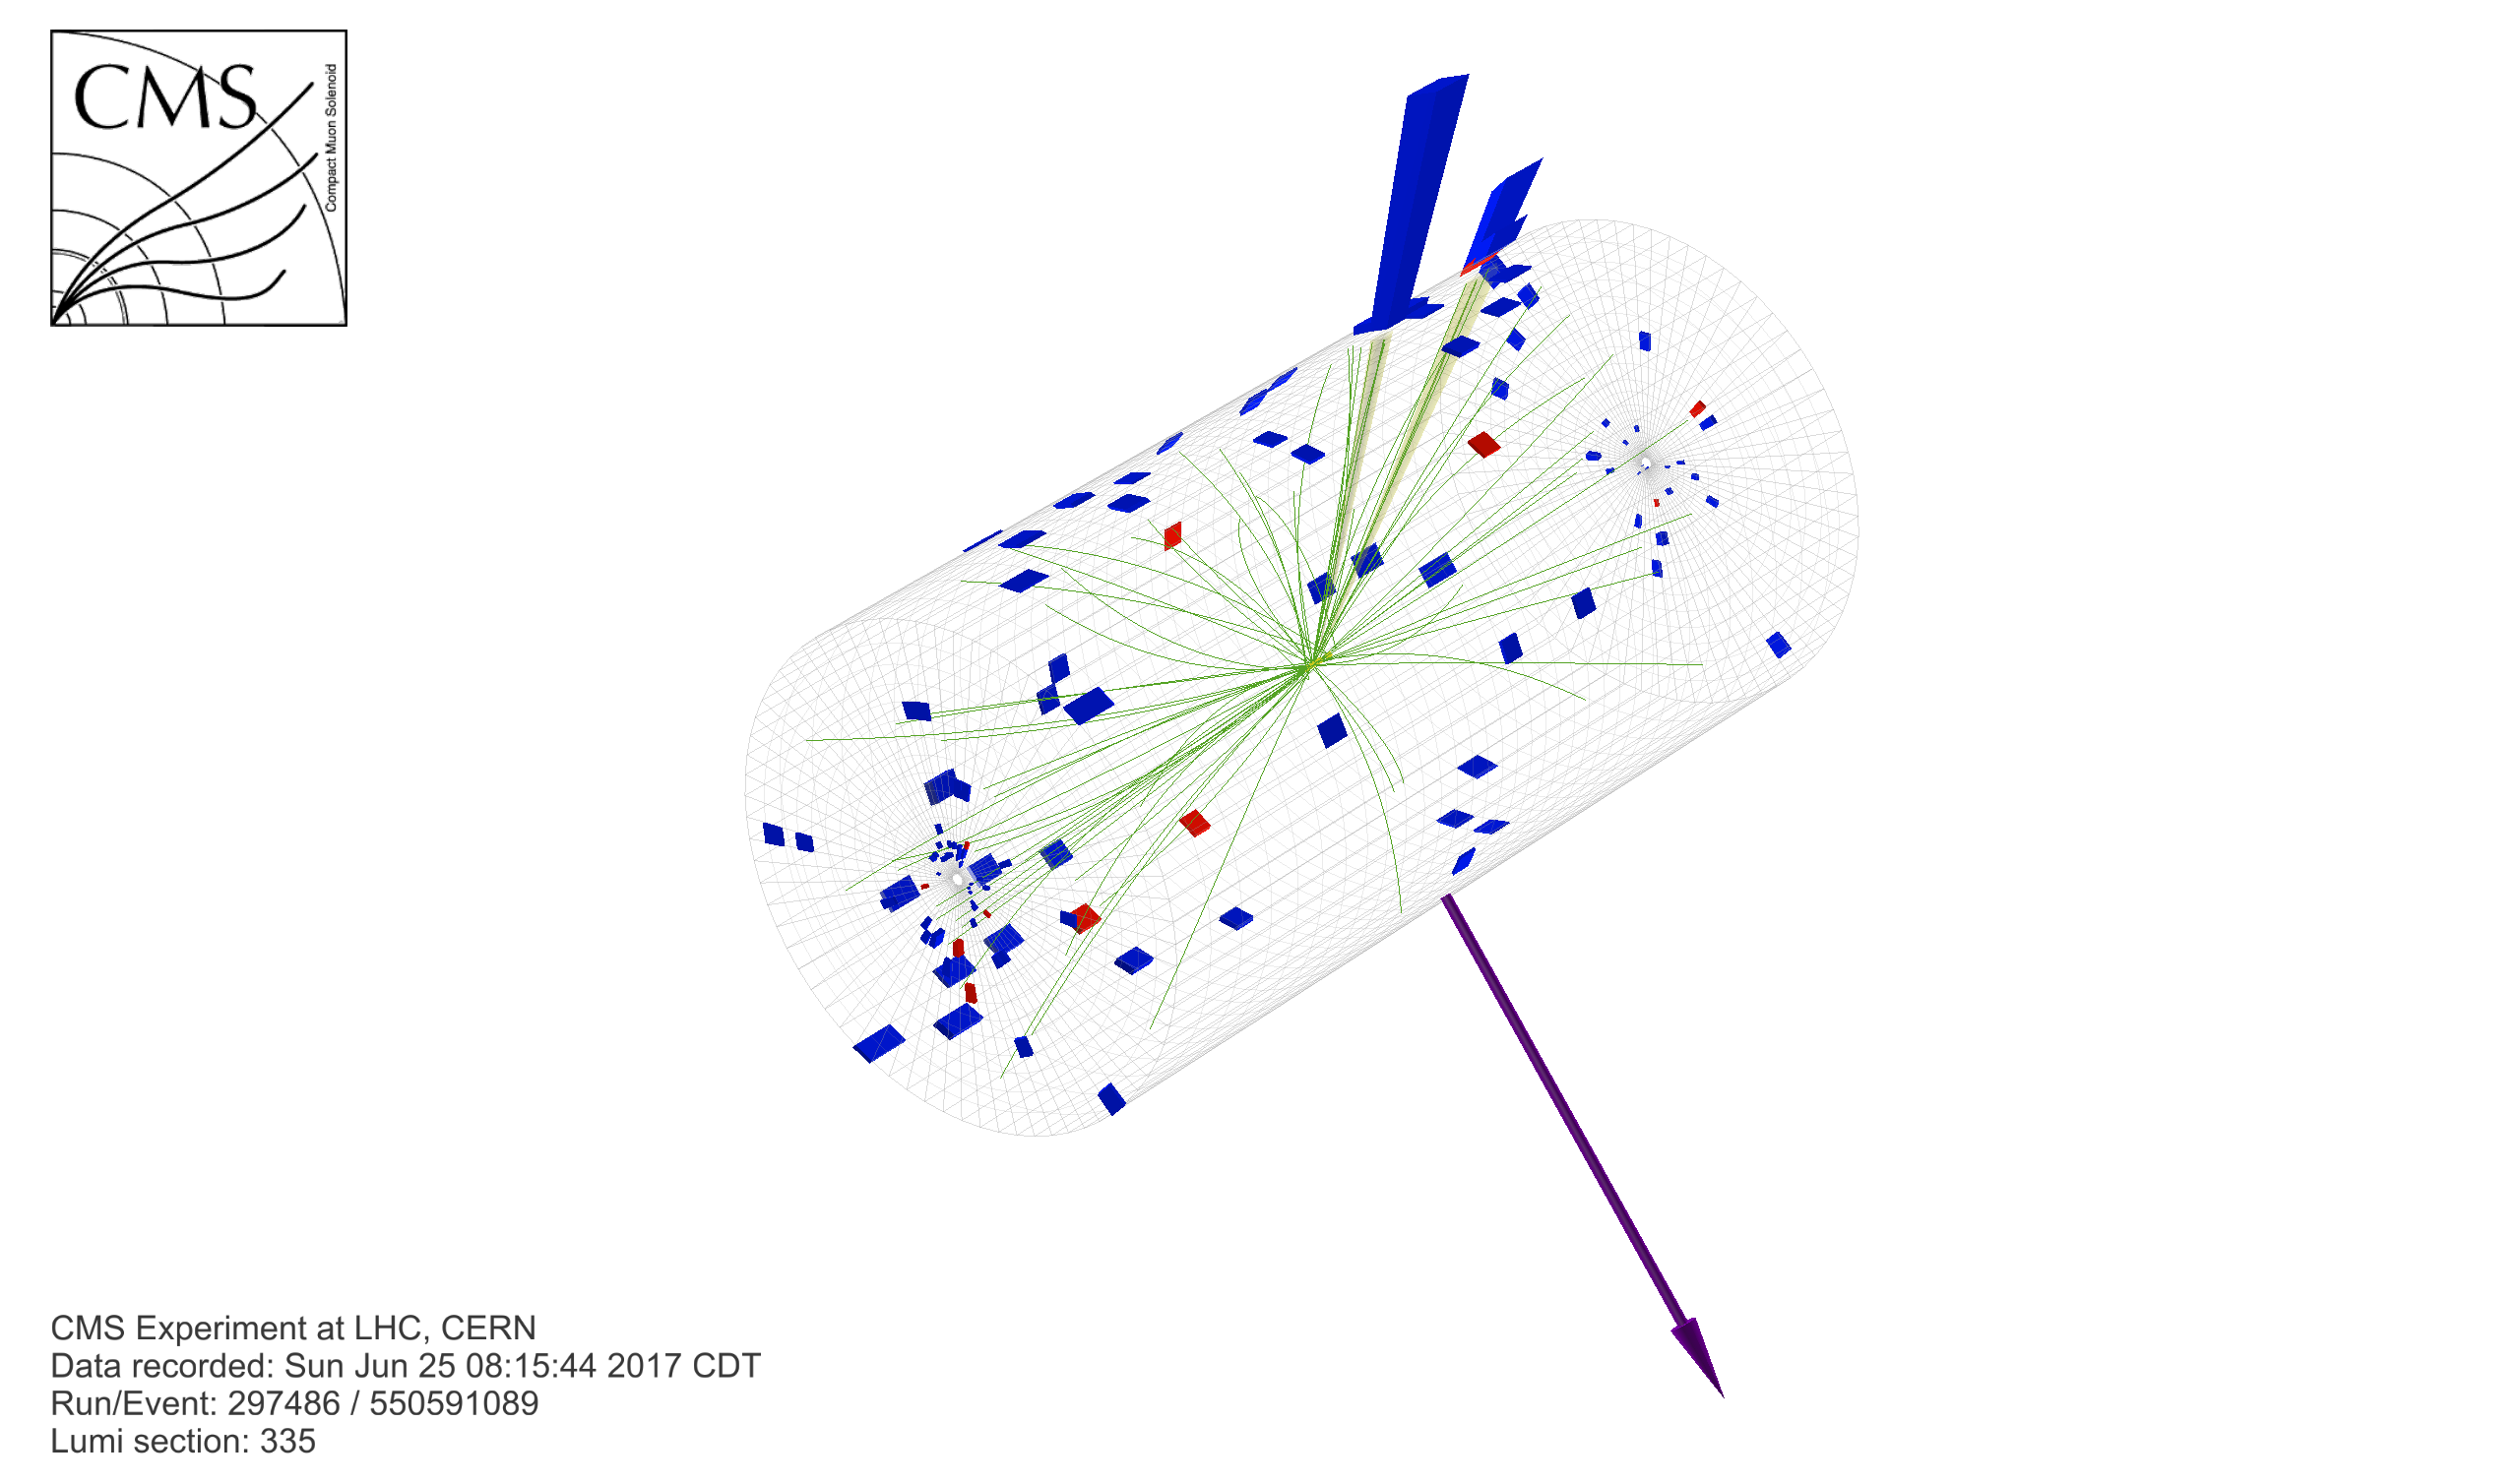
\includegraphics[width=\linewidth]{images/Znn_PerspXOZ_w}}
  }
  \mbox{
    \subfigure [] {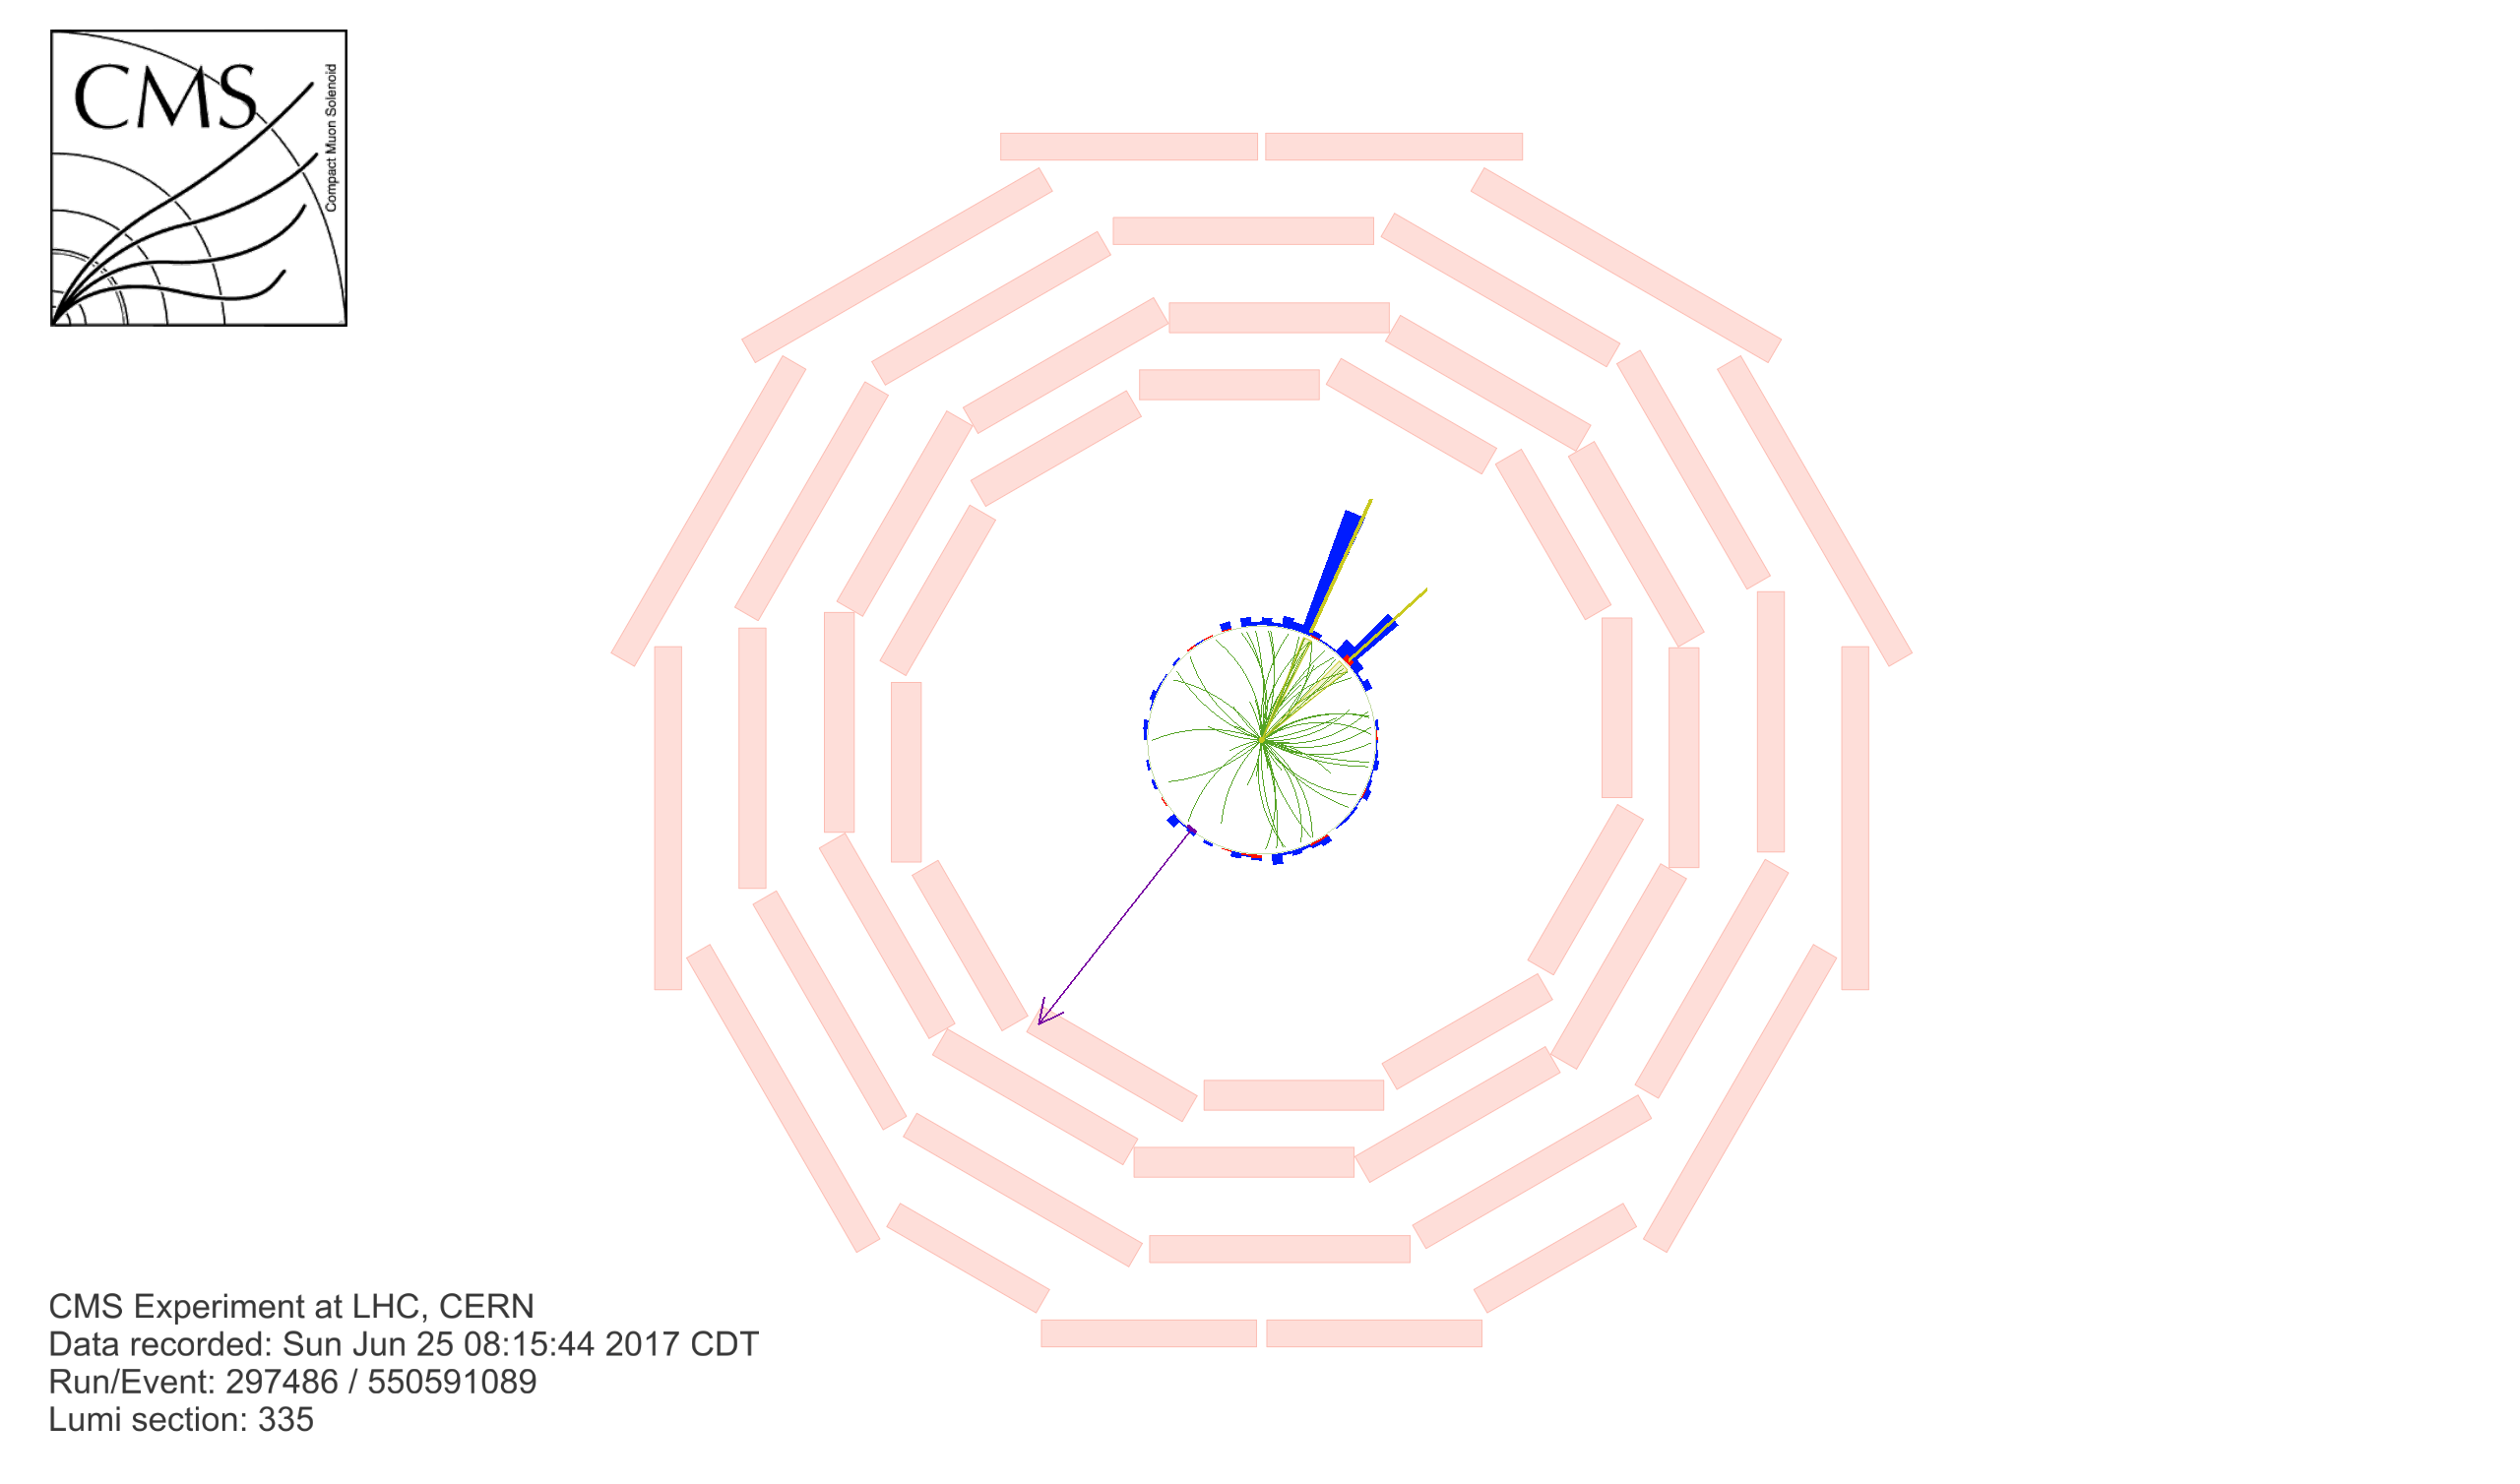
\includegraphics[width=0.5\linewidth]{images/Znn_rhophi_w}}
    \subfigure [] {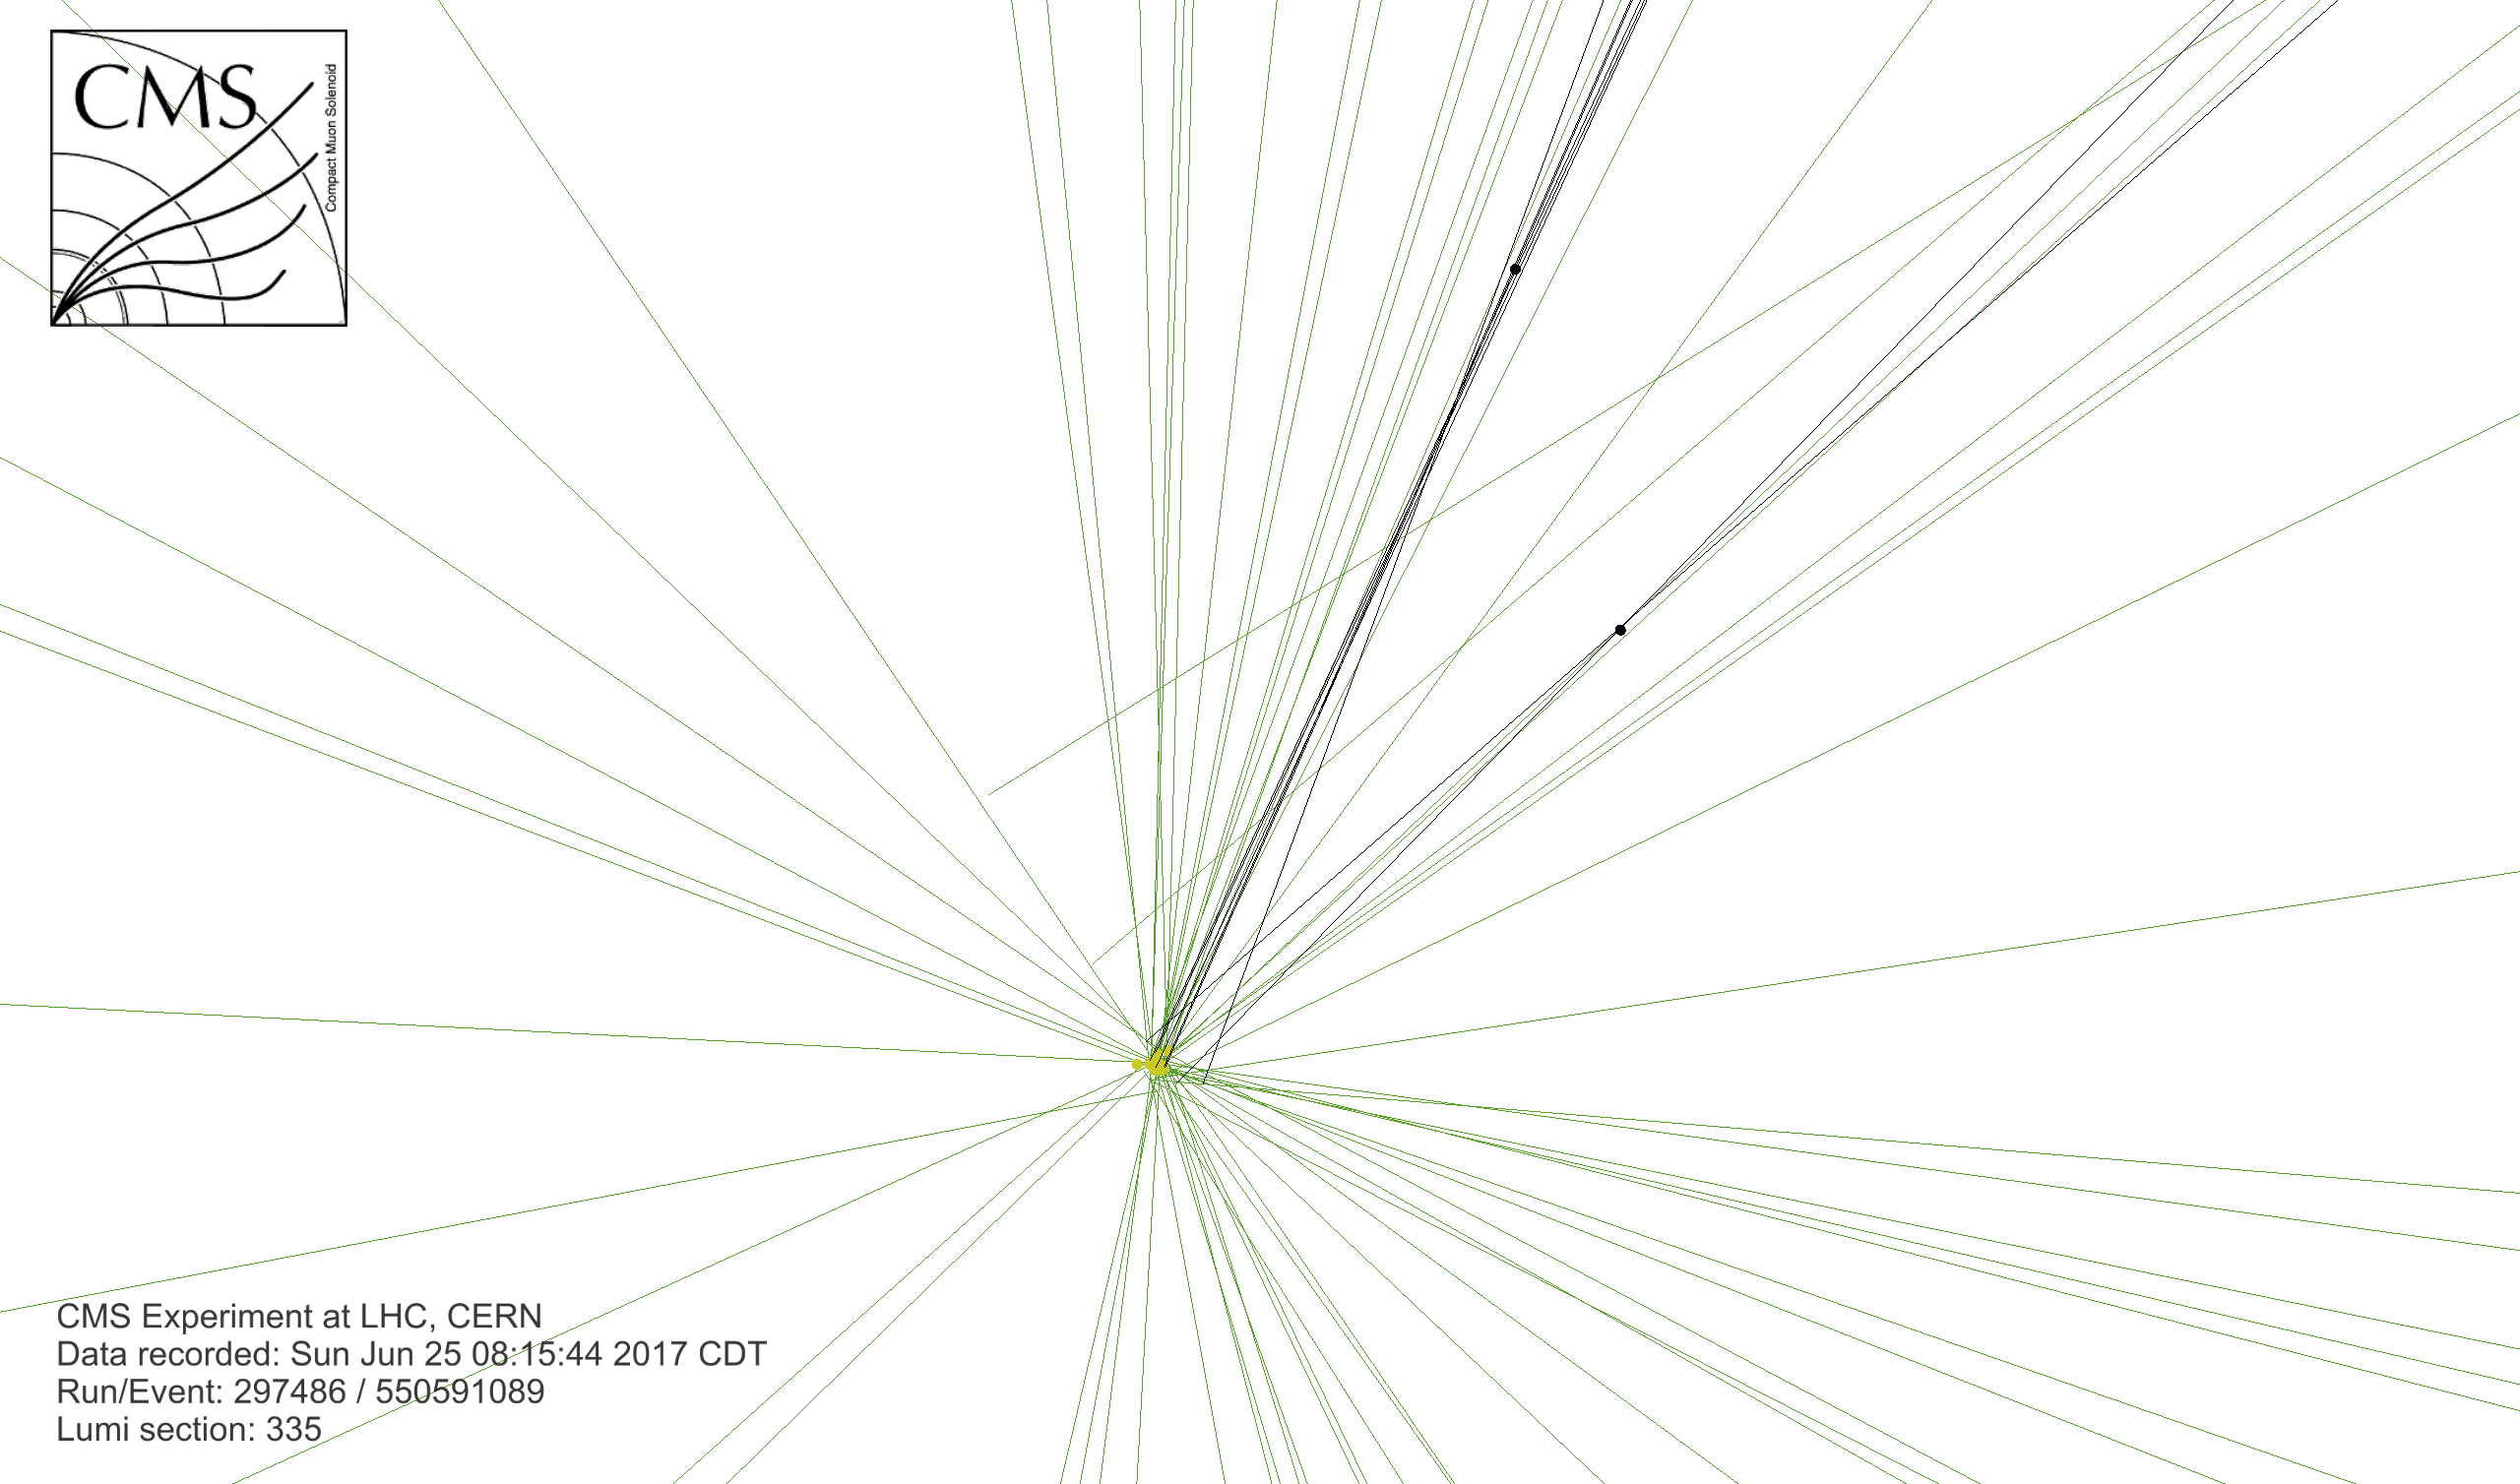
\includegraphics[width=0.5\linewidth]{images/ZnnSV_rhophi_w}}
  }
  \caption[Event Display for \ZnnHbb\ Candidate]{The event display for a candidate \ZnnHbb\ event A) from a 3D perspective view; B) projected onto the \textit{xy}-plane; and C) projected onto the \textit{xy}-plane and zoomed in on the interaction point. The purple arrow represents the missing transverse momentum from the invisible leptonic decay of the \bosZ\ boson while the two yellow cones with their blue and red calorimeter towers represent the two \qrkb-jets from the decay of the Higgs boson. The secondary vertices of the \qrkb-jets and their associated tracks (black) are visible in C.}
  \label{fig:evt_disp_Znn}
\end{figure}

\begin{figure}[htbp]
  \centering
  \mbox{
    \subfigure [] {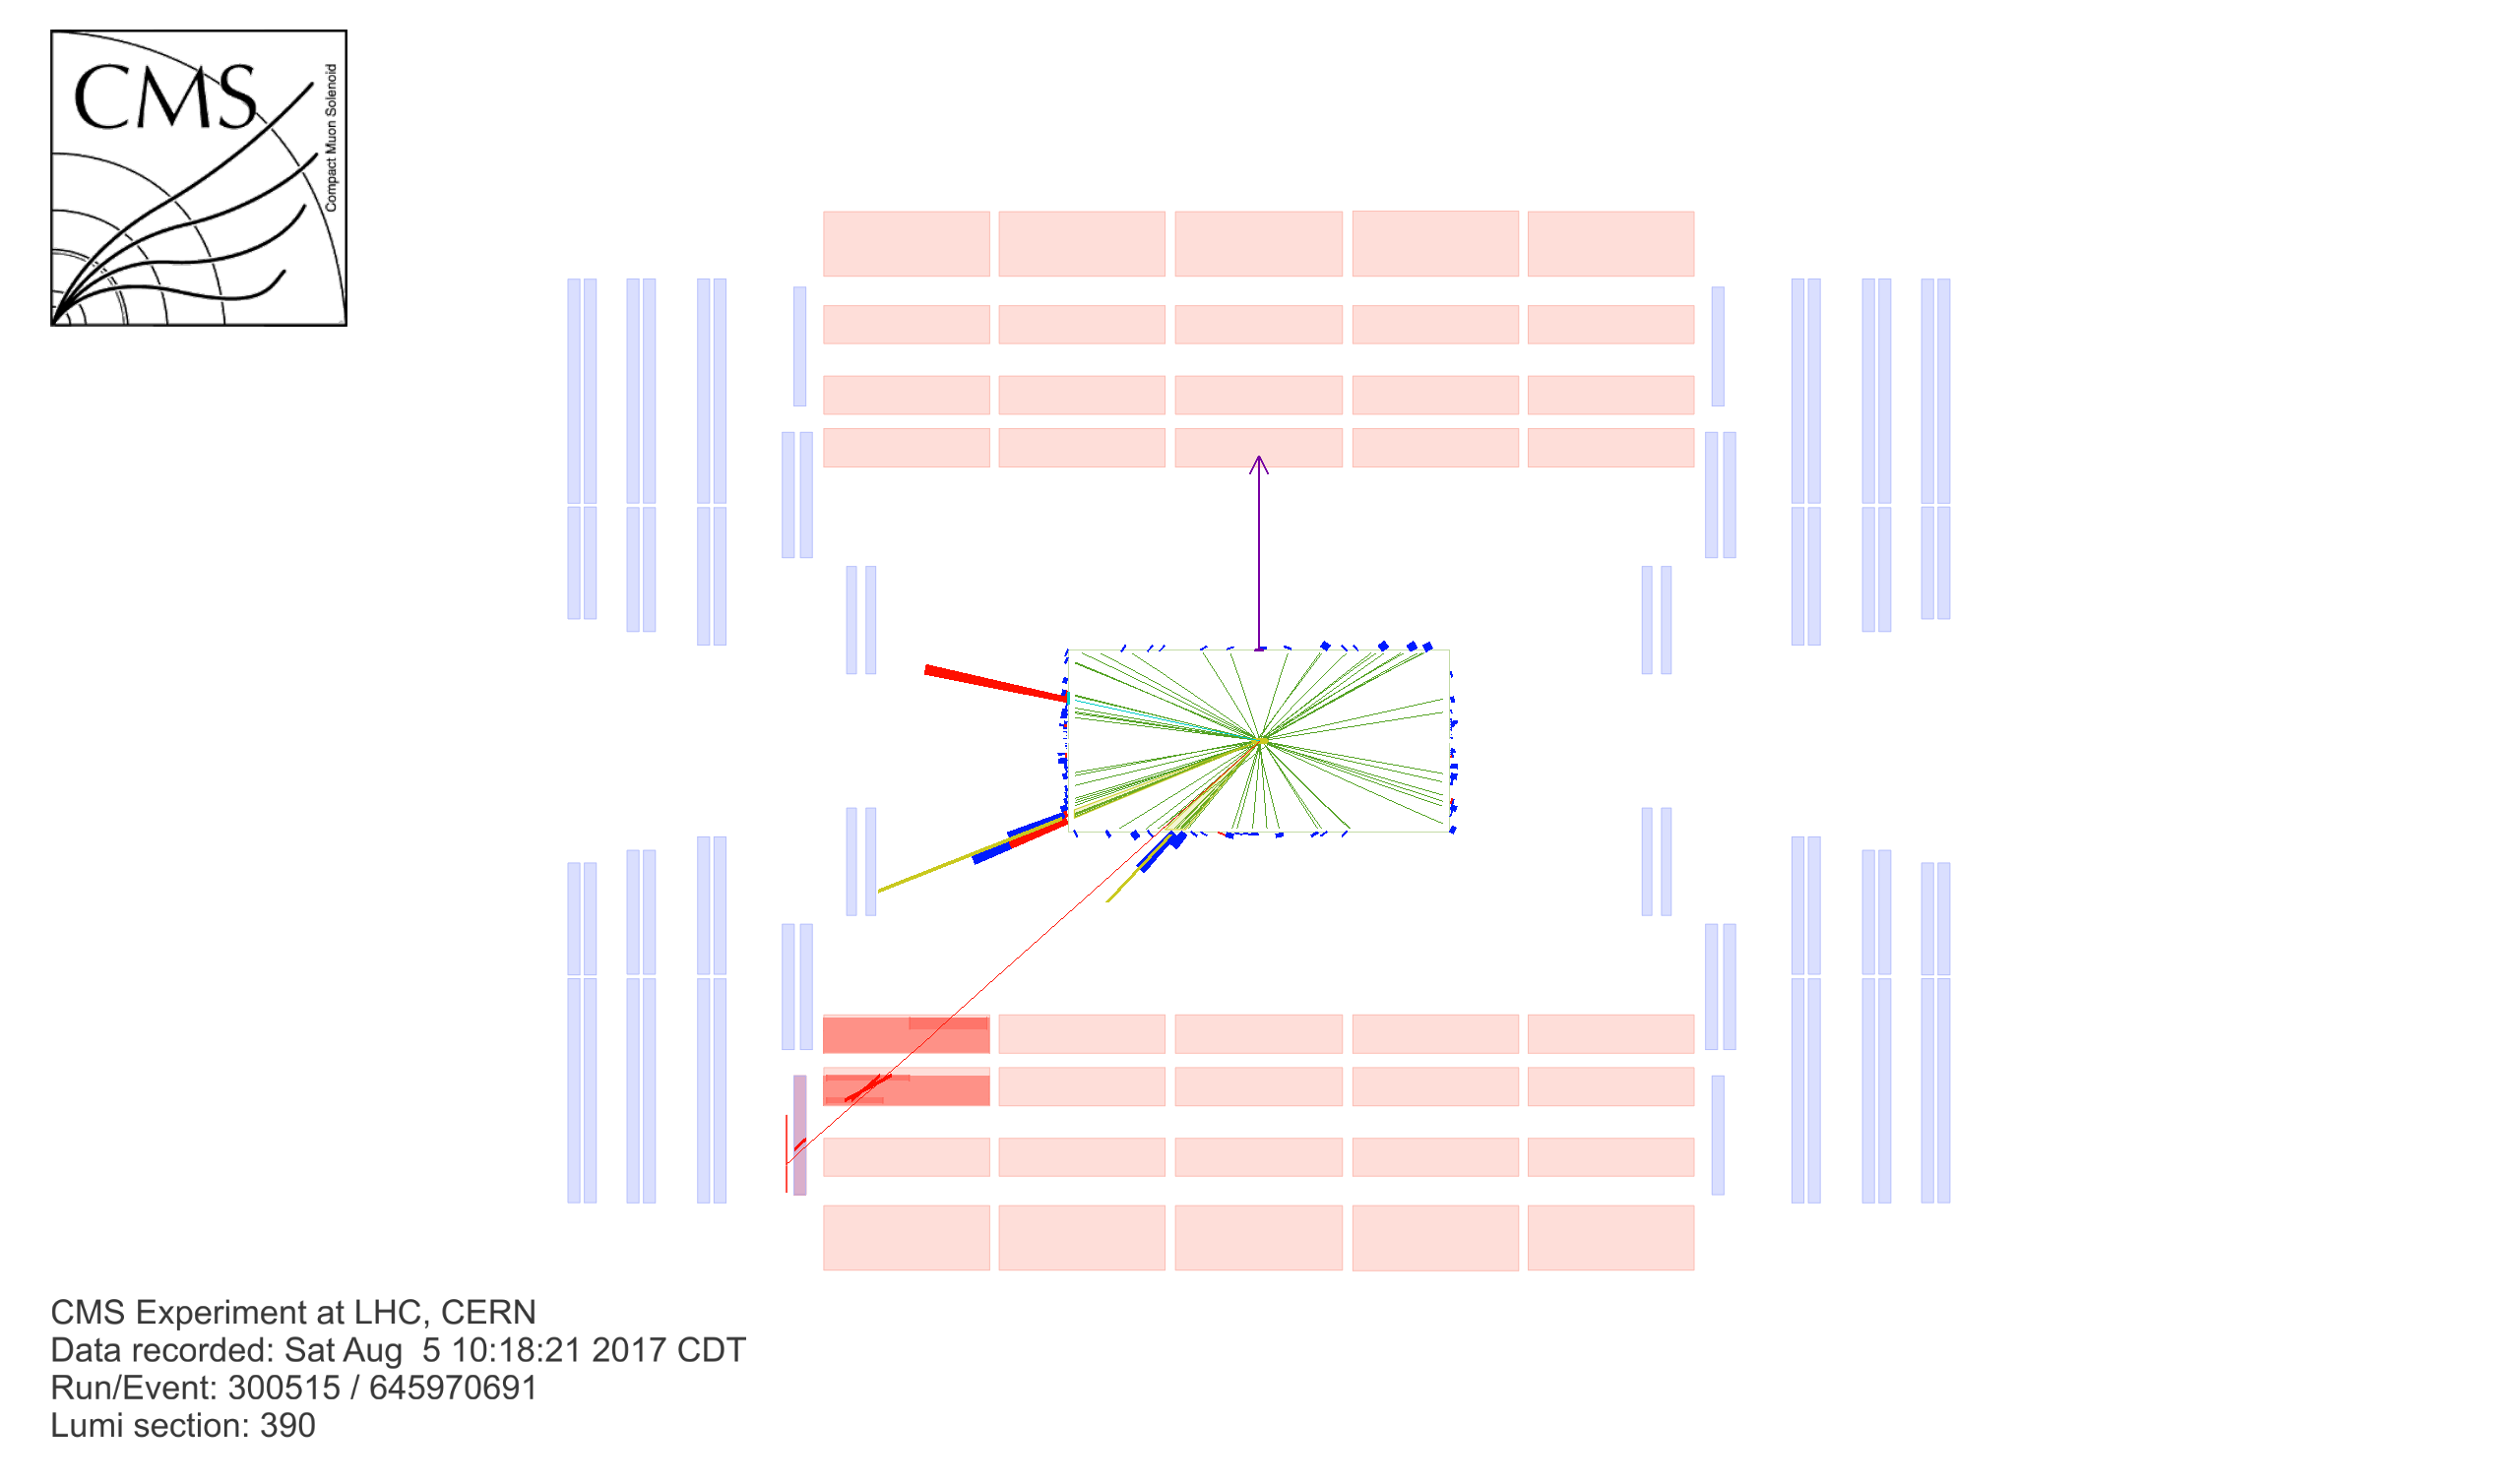
\includegraphics[width=\linewidth]{images/Wen_rhoz_w}}
  }
  \mbox{
    \subfigure [] {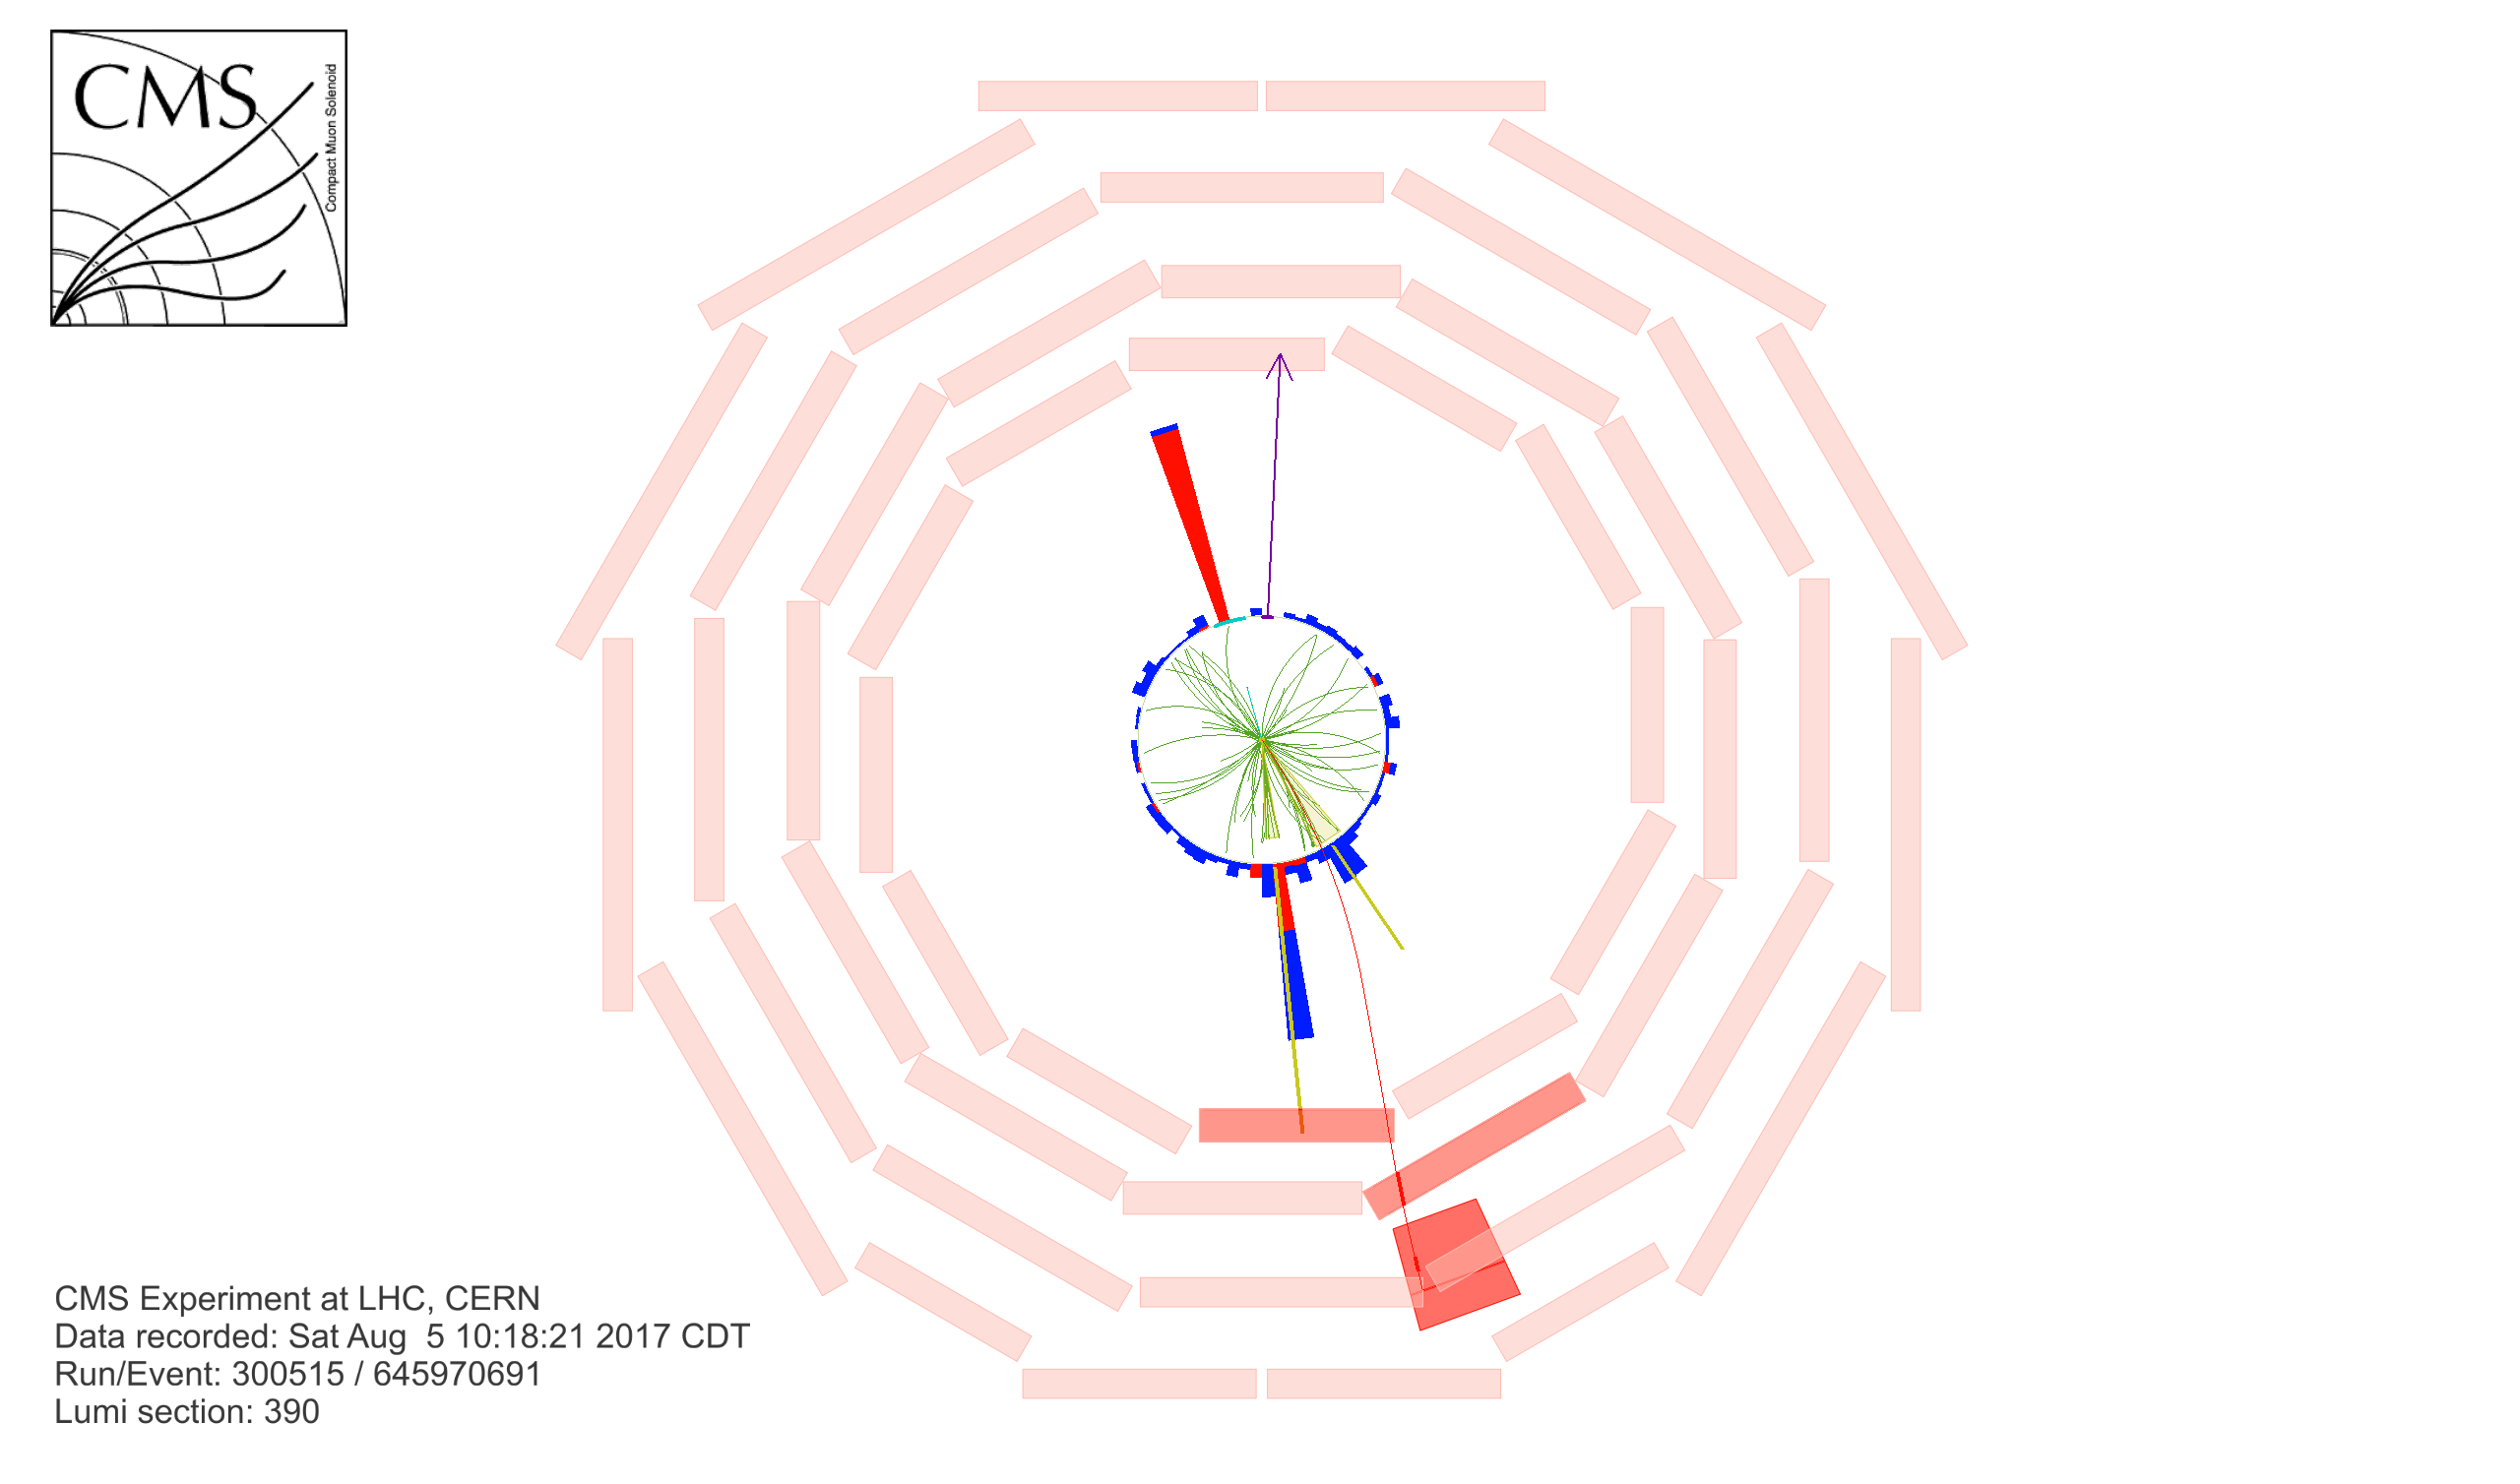
\includegraphics[width=0.5\linewidth]{images/Wen_rhophi_w}}
    \subfigure [] {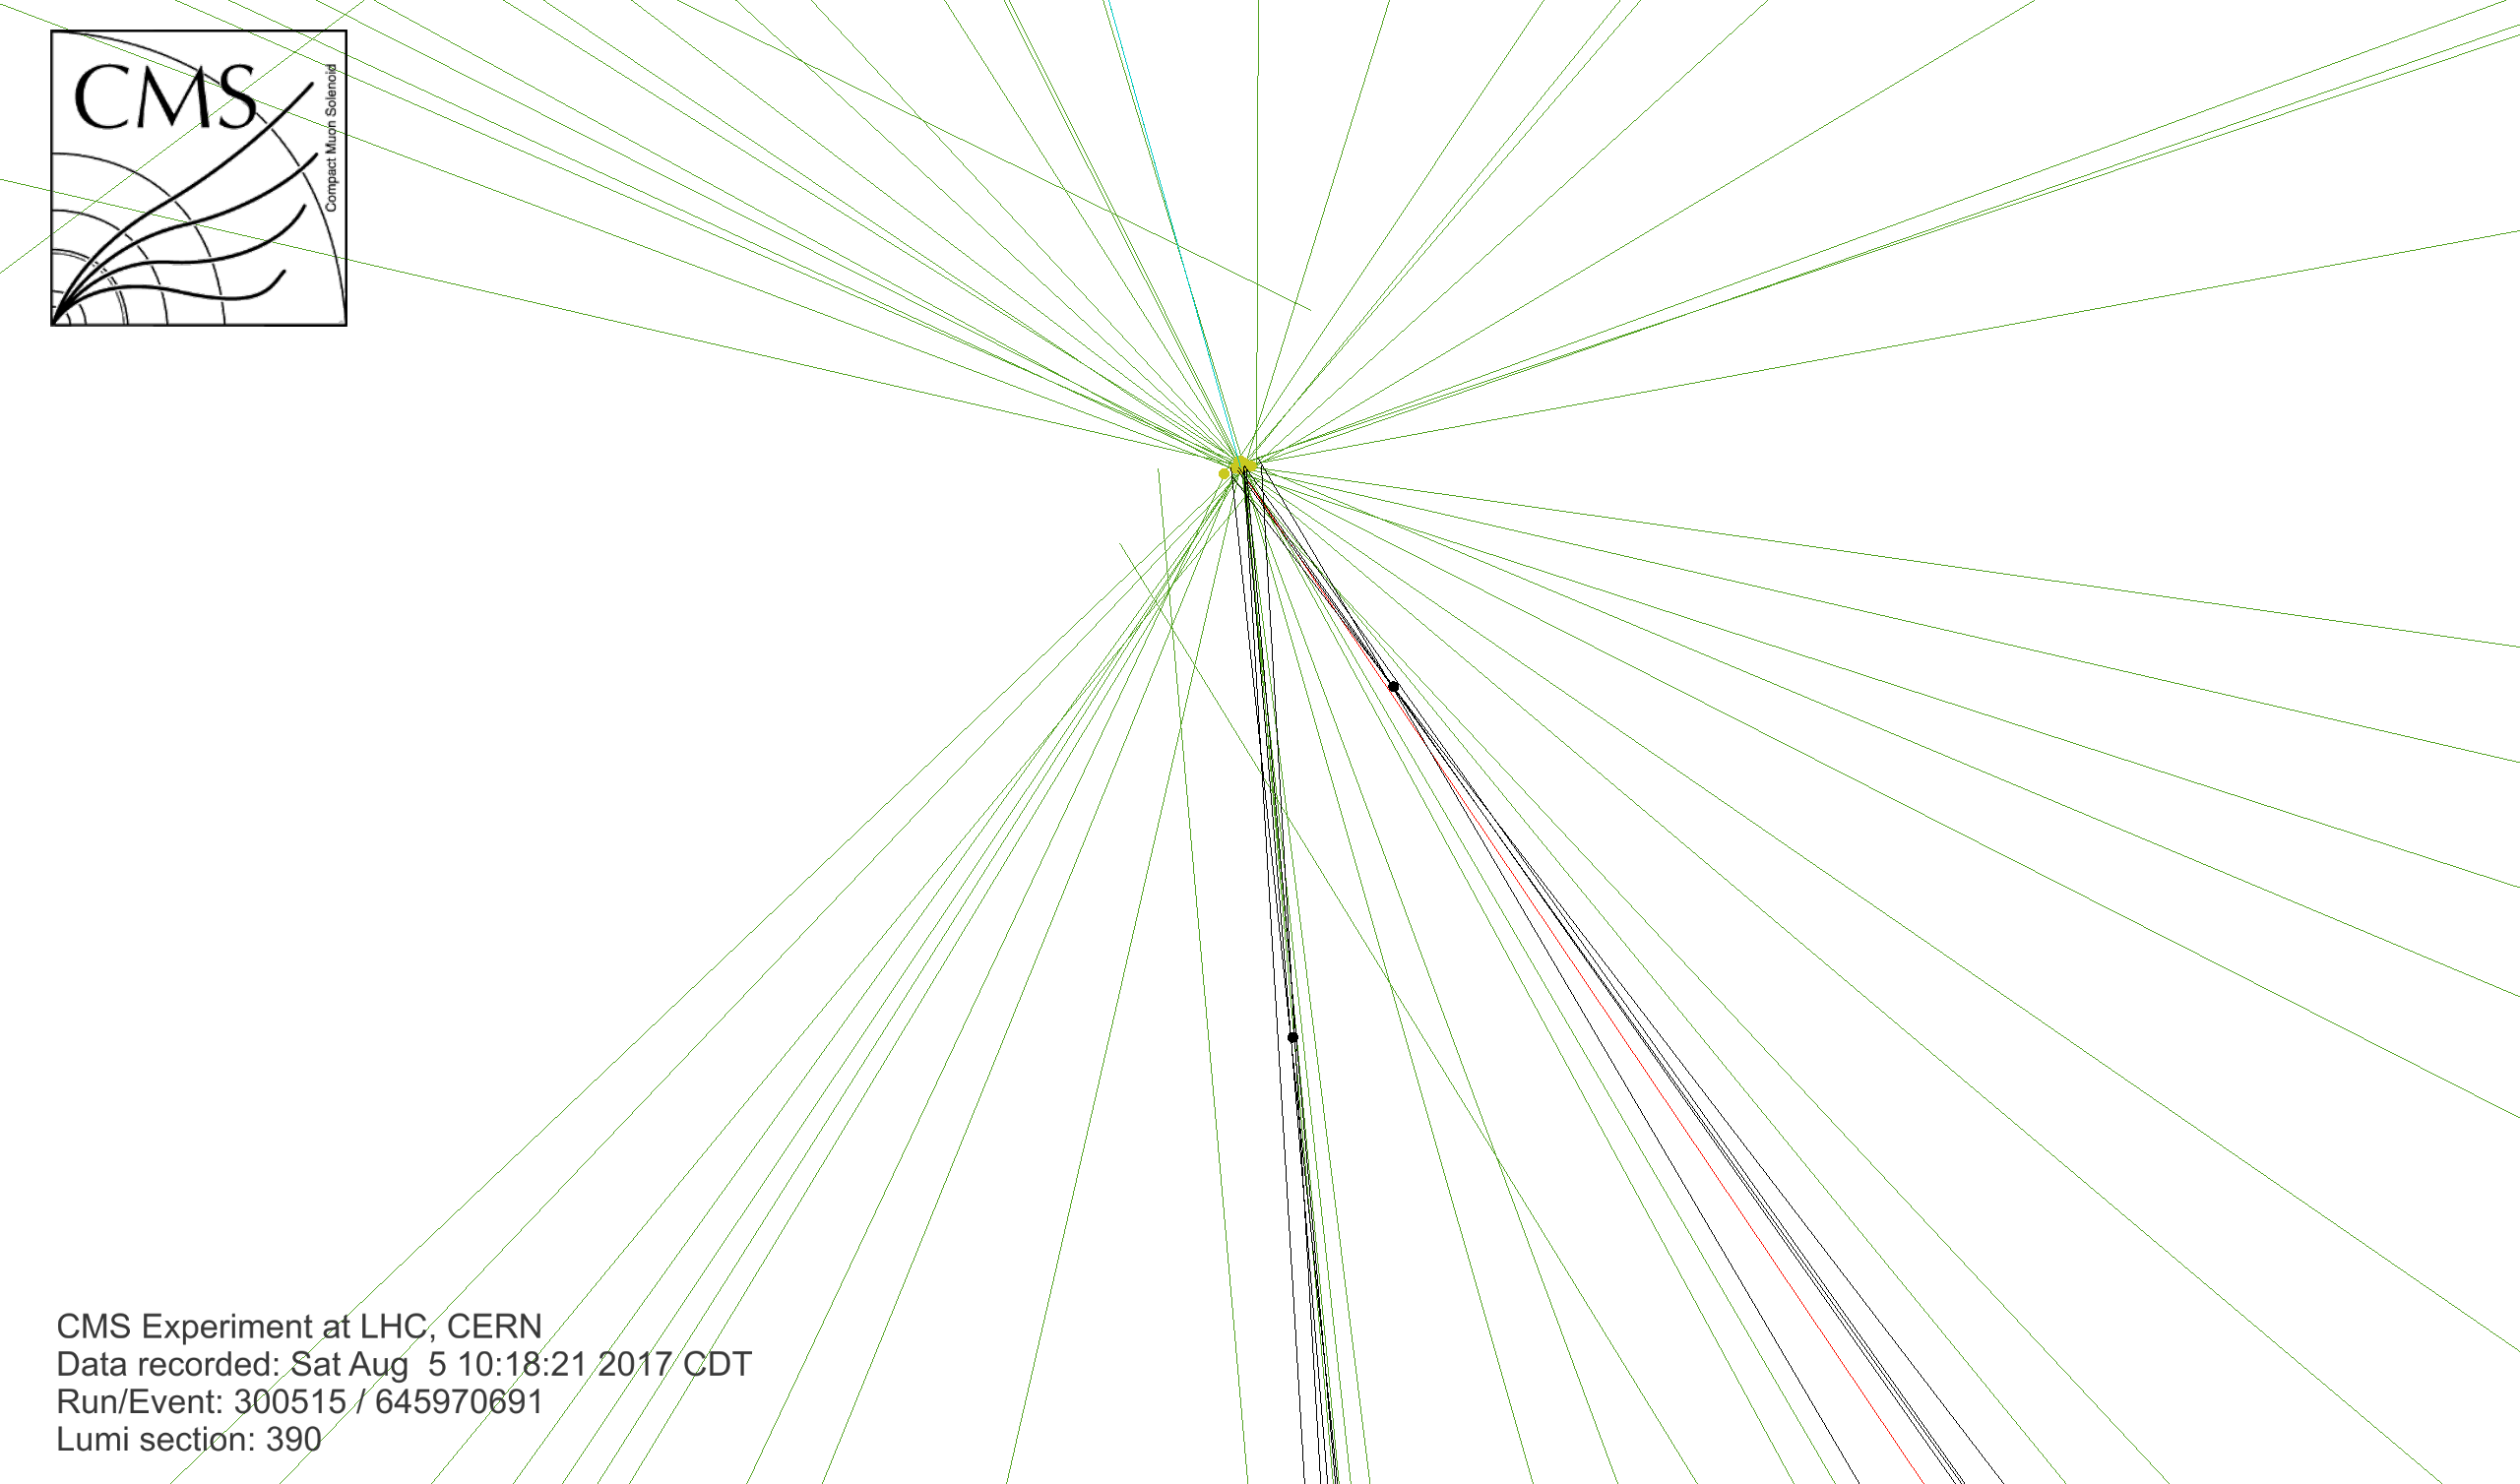
\includegraphics[width=0.5\linewidth]{images/WenSV_rhophi_w}}
  }
  \caption[Event Display for \WenHbb\ Candidate]{The event display for a candidate \WenHbb\ event A) projected onto the \textit{xz}-plane; B) projected onto the \textit{xy}-plane; and C) projected onto the \textit{xy}-plane and zoomed in on the interaction point. The cyan track leading to a red calorimeter tower and the purple arrow represent the electron and the missing transverse momentum from the leptonic decay of the \bosW\ boson, respectively, while the two yellow cones with their blue and red calorimeter towers represent the two \qrkb-jets from the decay of the Higgs boson. The secondary vertices of the \qrkb-jets and their associated tracks (black) are visible in C. The red track associated with one of the \qrkb-jets is likely a muon resulting from a semi-leptonic decay of the \qrkb-hadron.}
  \label{fig:evt_disp_Wen}
\end{figure}

\begin{figure}[htbp]
  \centering
  \mbox{
    \subfigure [] {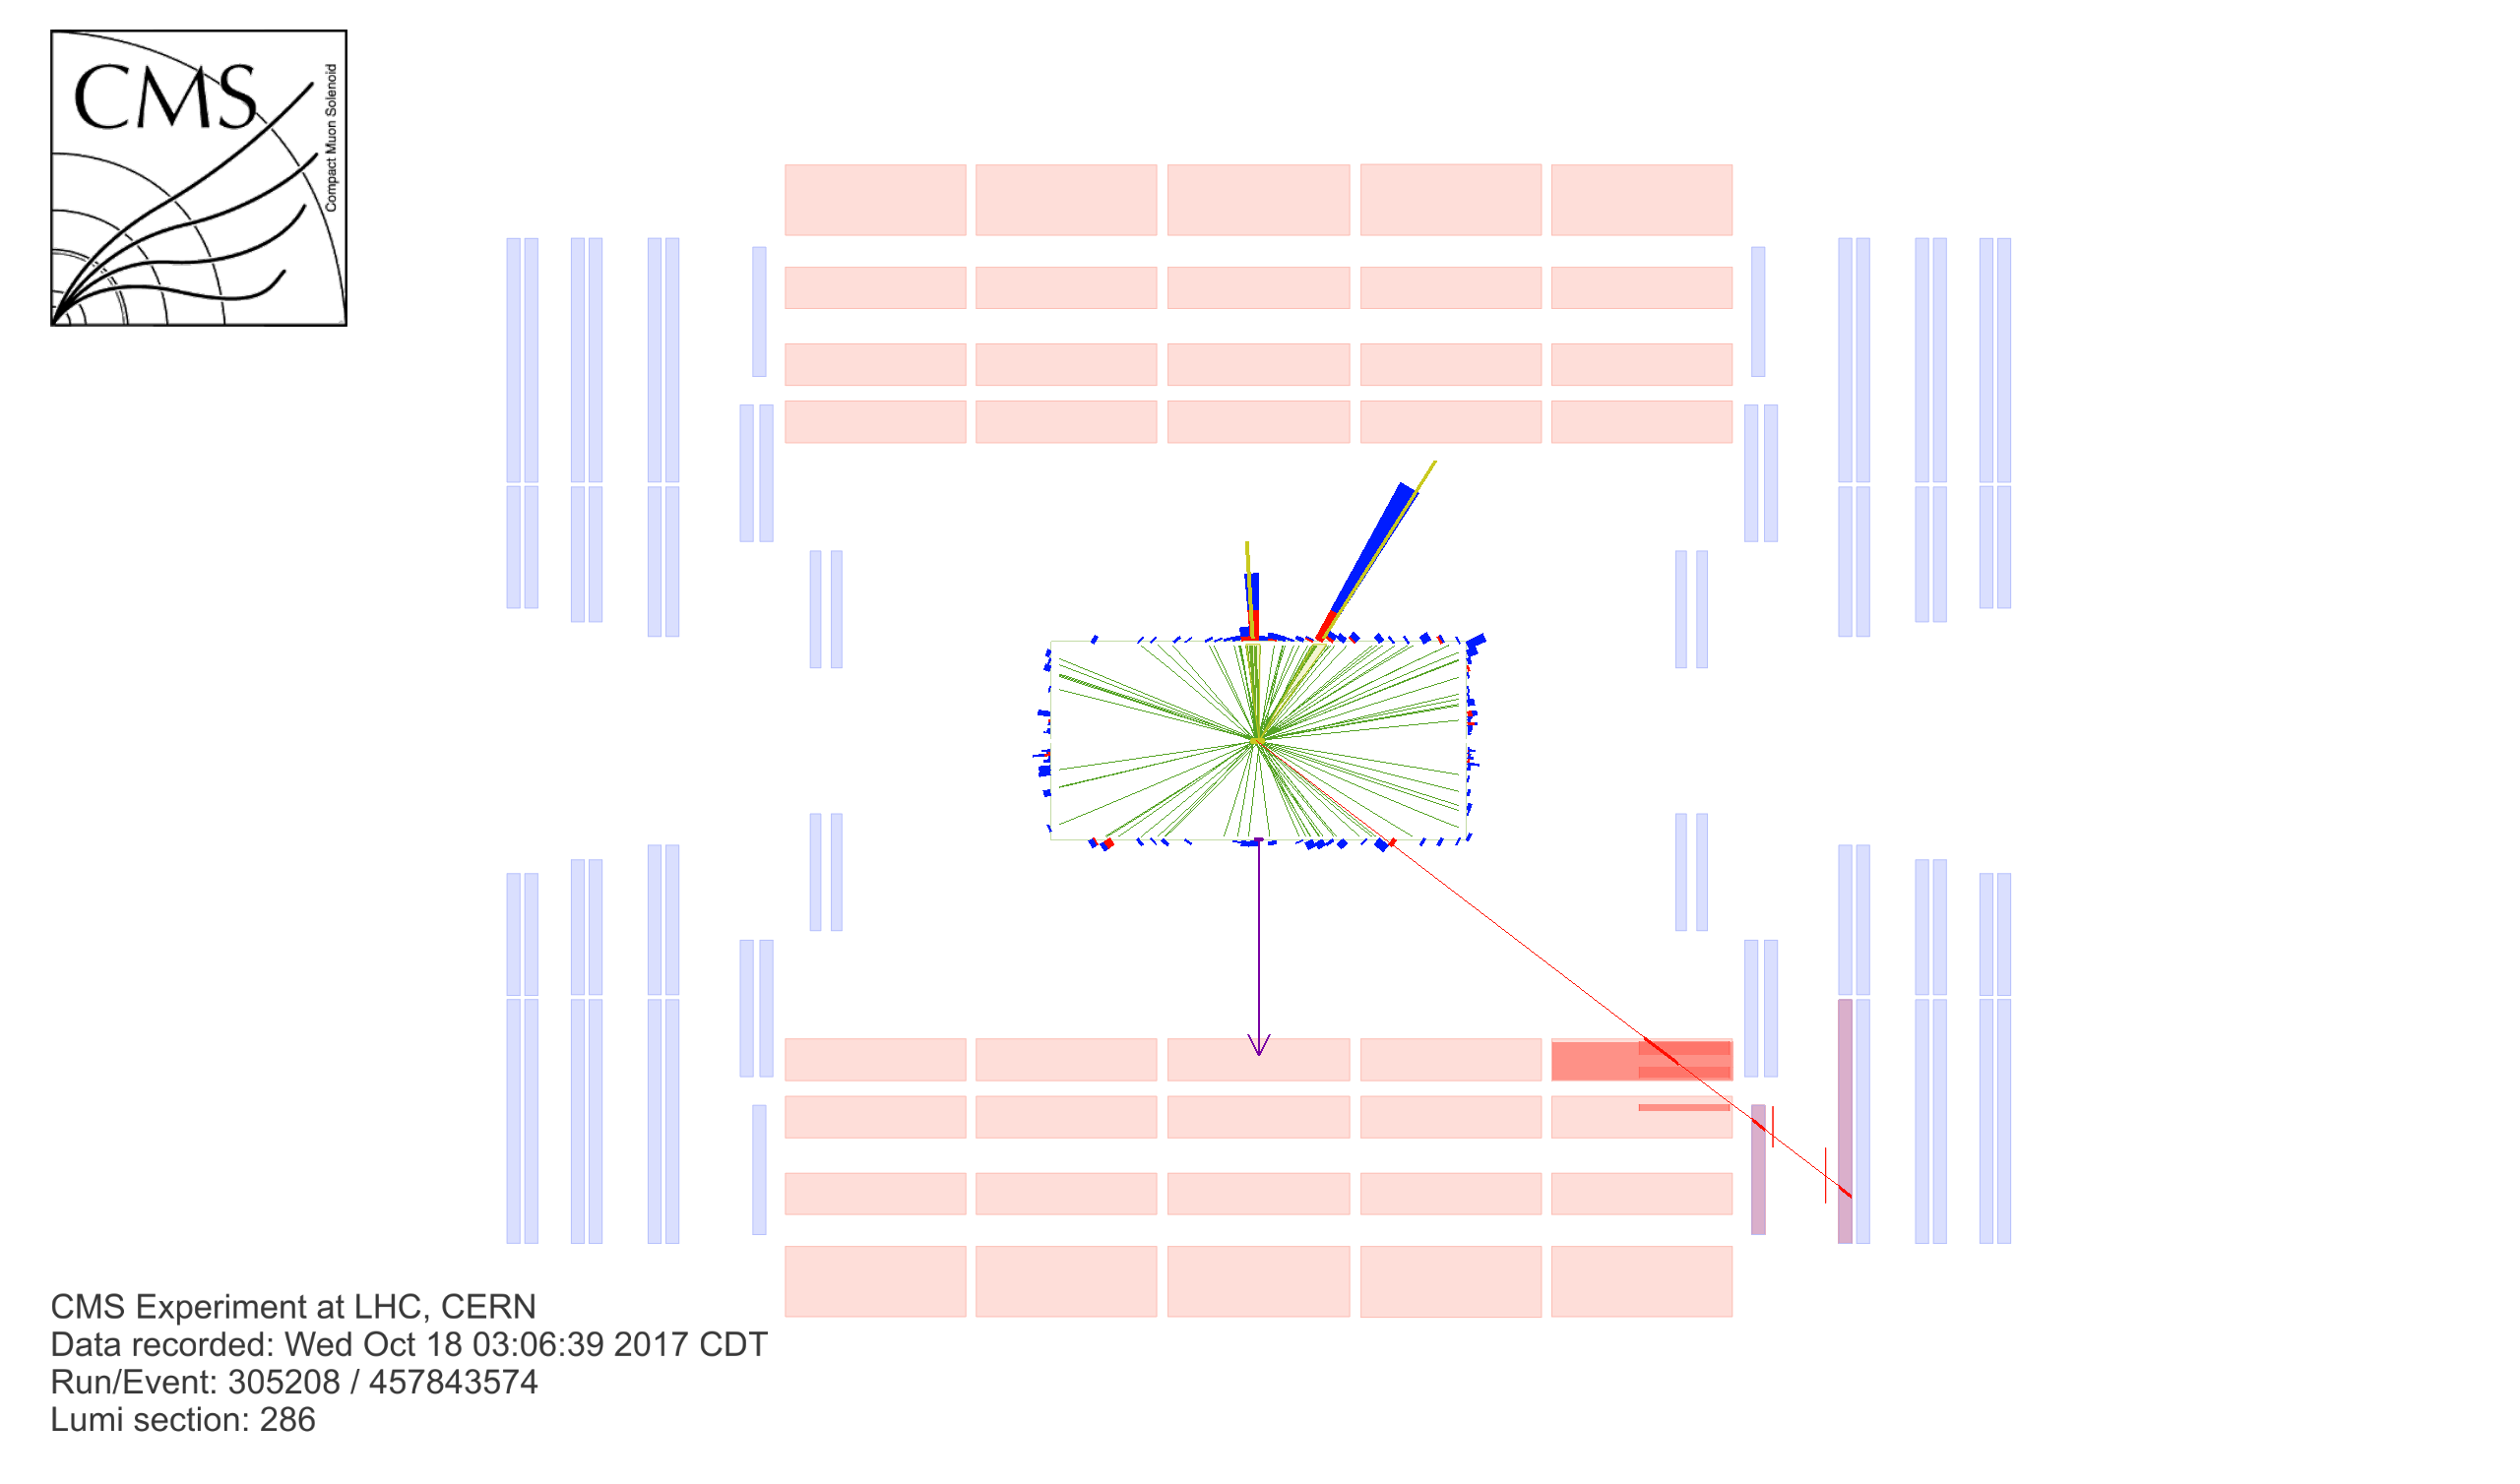
\includegraphics[width=\linewidth]{images/Wmn_rhoz_w}}
  }
  \mbox{
    \subfigure [] {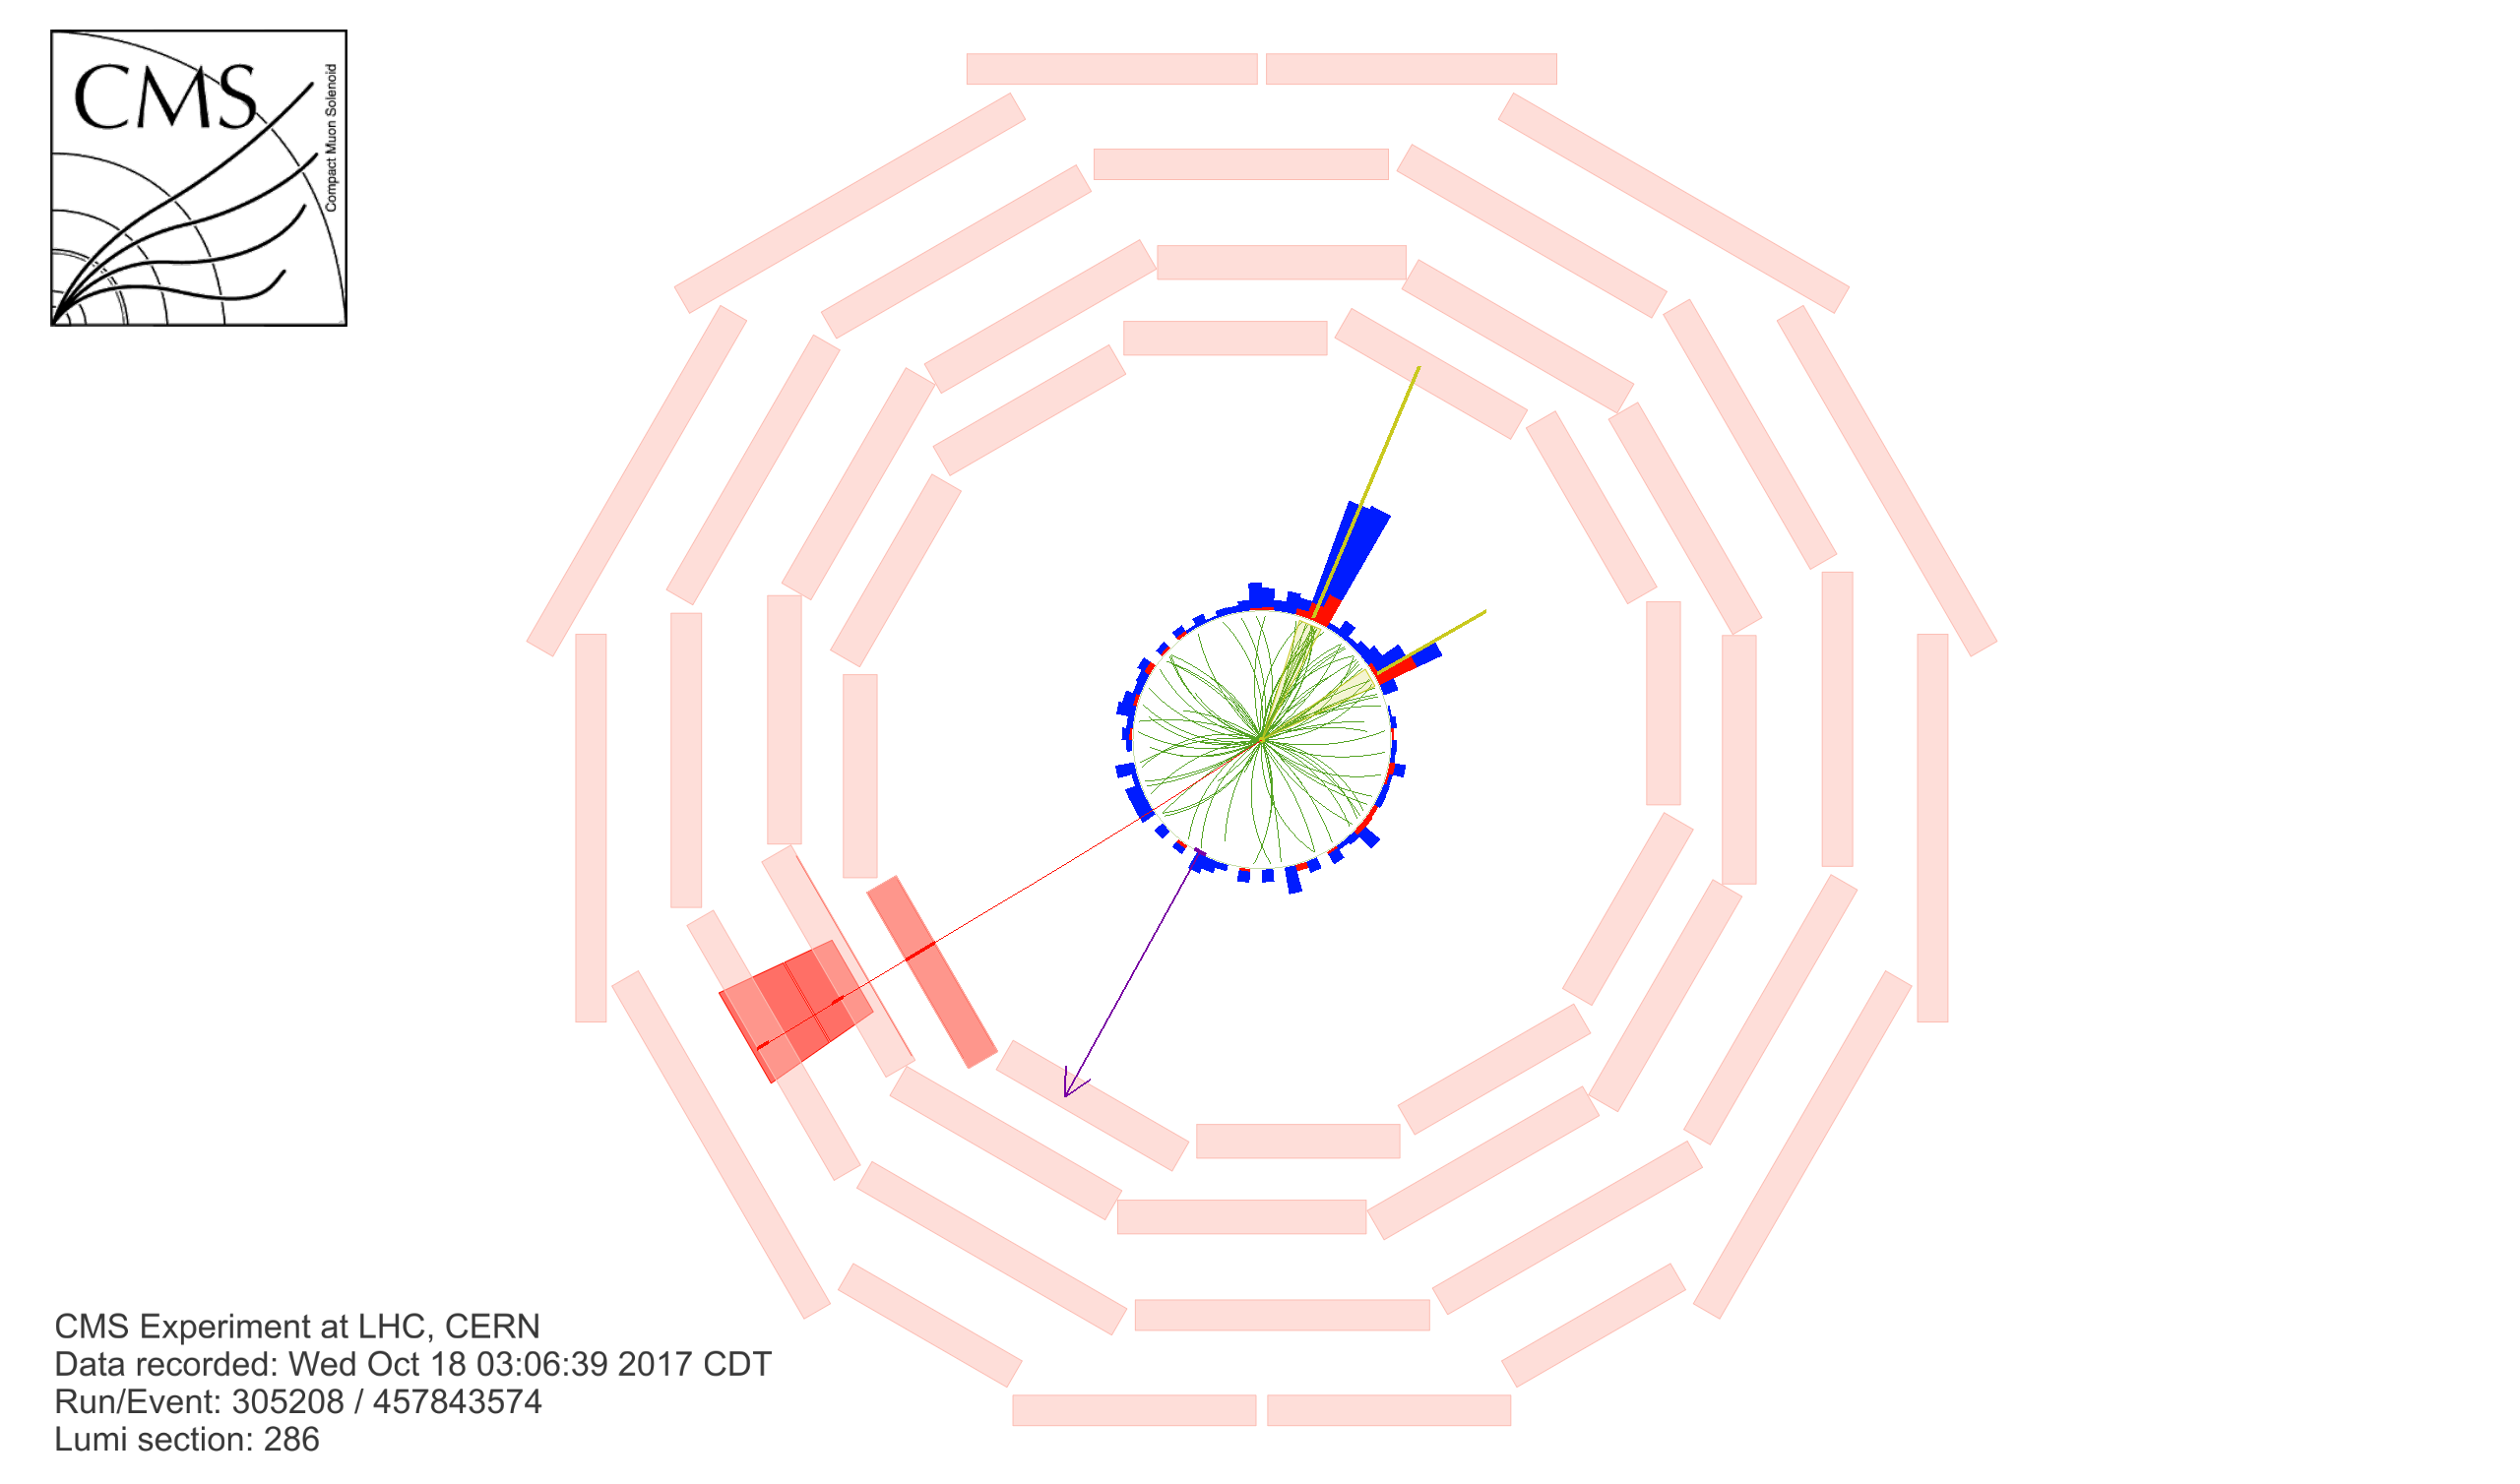
\includegraphics[width=0.5\linewidth]{images/Wmn_rhophi_w}}
    \subfigure [] {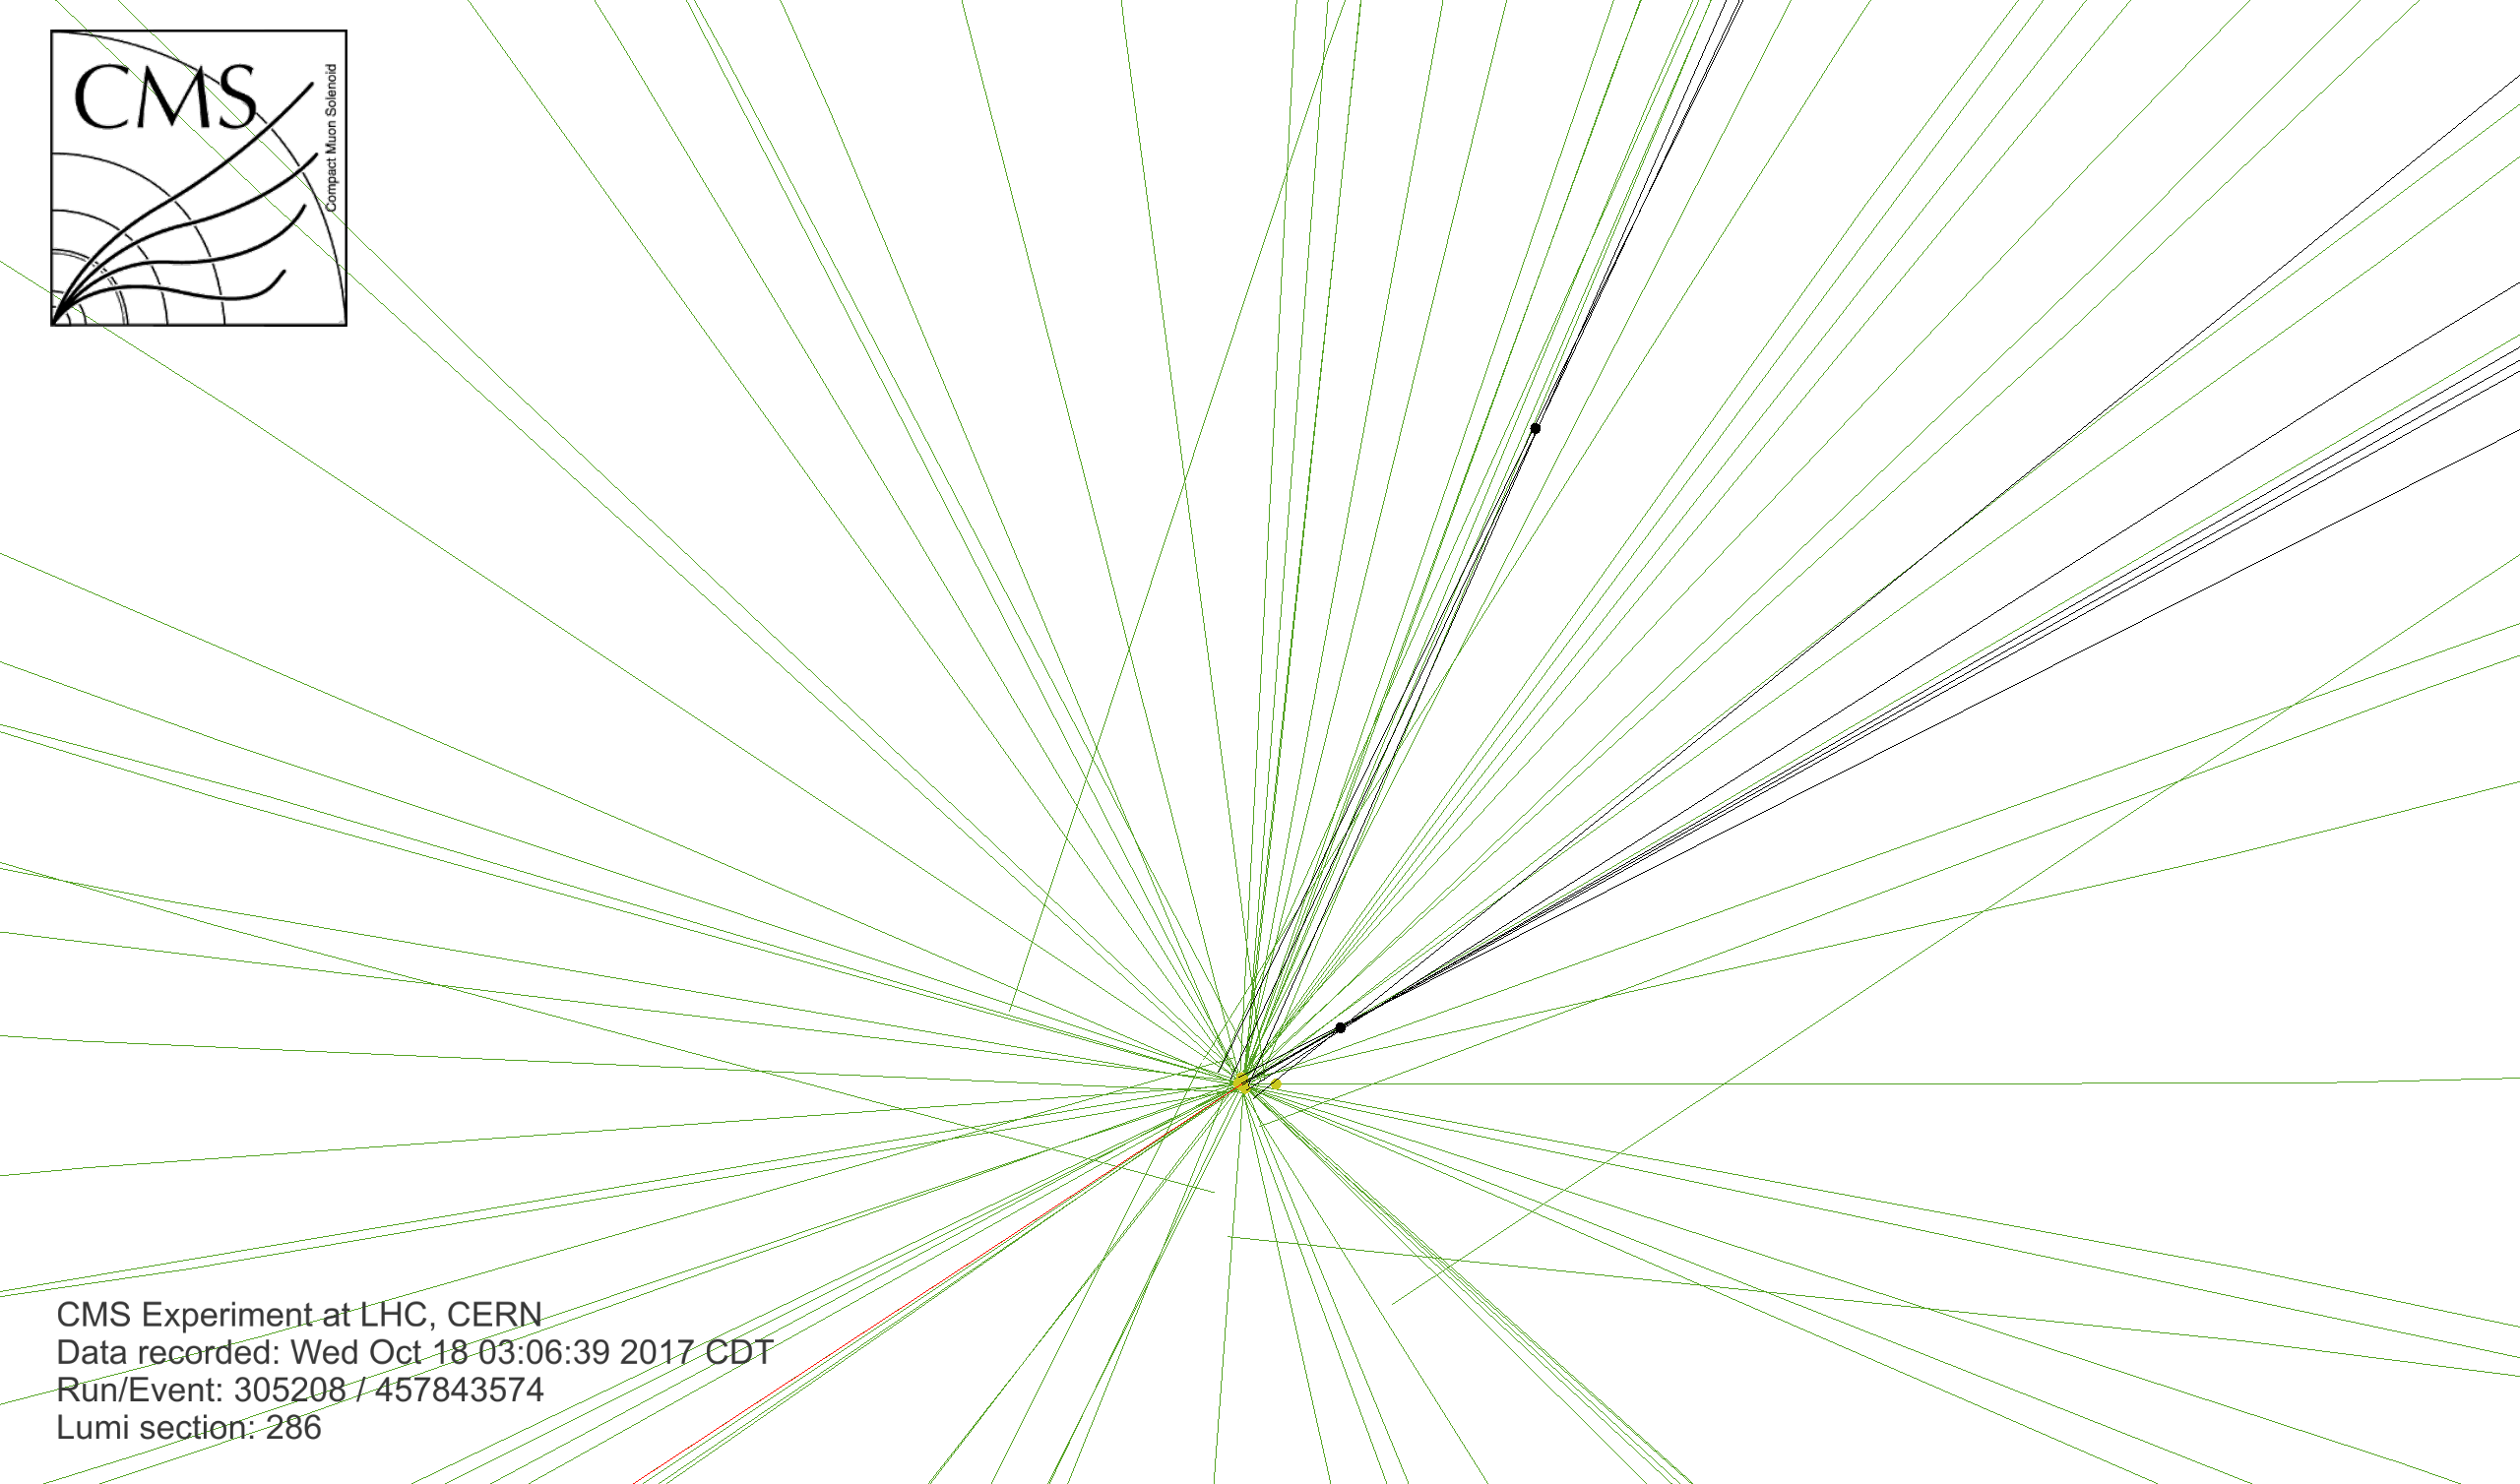
\includegraphics[width=0.5\linewidth]{images/WmnSV_rhophi_w}}
  }
  \caption[Event Display for \WmnHbb\ Candidate]{The event display for a candidate \WmnHbb\ event A) projected onto the \textit{xz}-plane; B) projected onto the \textit{xy}-plane; and C) projected onto the \textit{xy}-plane and zoomed onto the interaction point. The red track and the purple arrow represent the muon and the missing transverse momentum from the leptonic decay of the \bosW\ boson, respectively, while the two yellow cones with their blue and red calorimeter towers represent the two \qrkb-jets from the decay of the Higgs boson. The secondary vertices of the \qrkb-jets and their associated tracks (black) are visible in C.}
  \label{fig:evt_disp_Wmn}
\end{figure}

\begin{figure}[htbp]
  \centering
  \mbox{
    \subfigure [] {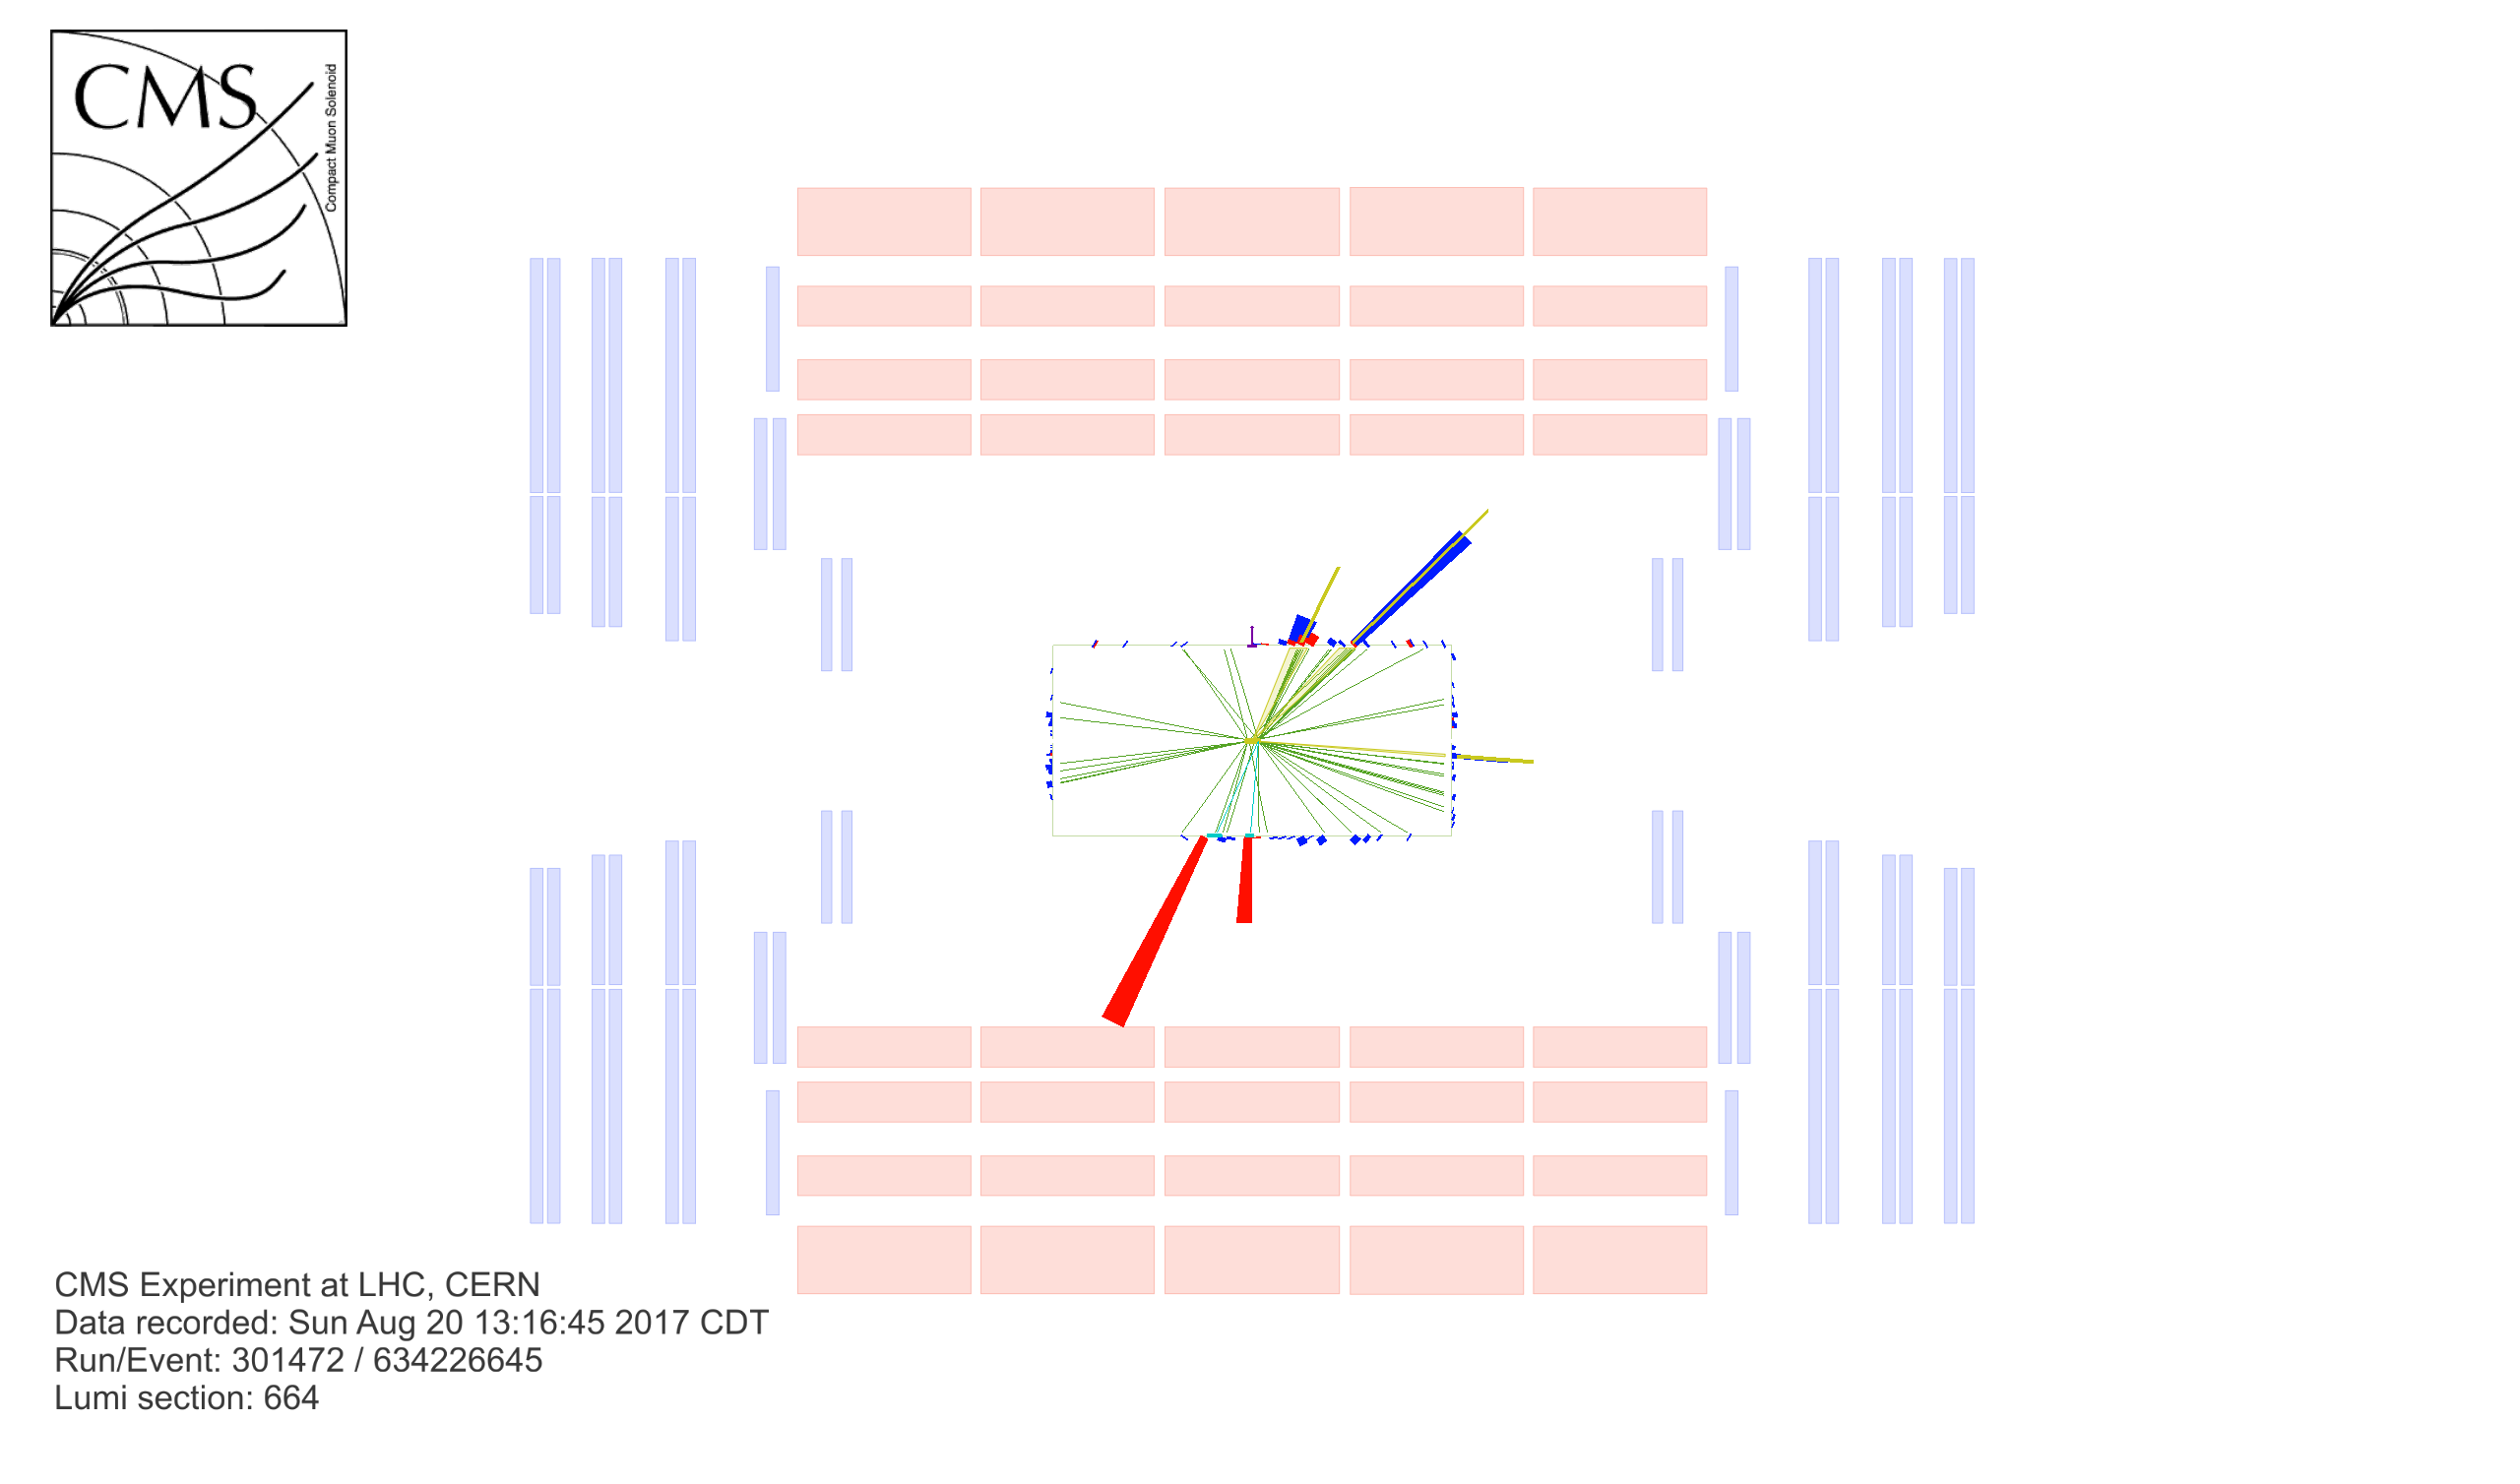
\includegraphics[width=\linewidth]{images/Zee_rhoz_w}}
  }
  \mbox{
    \subfigure [] {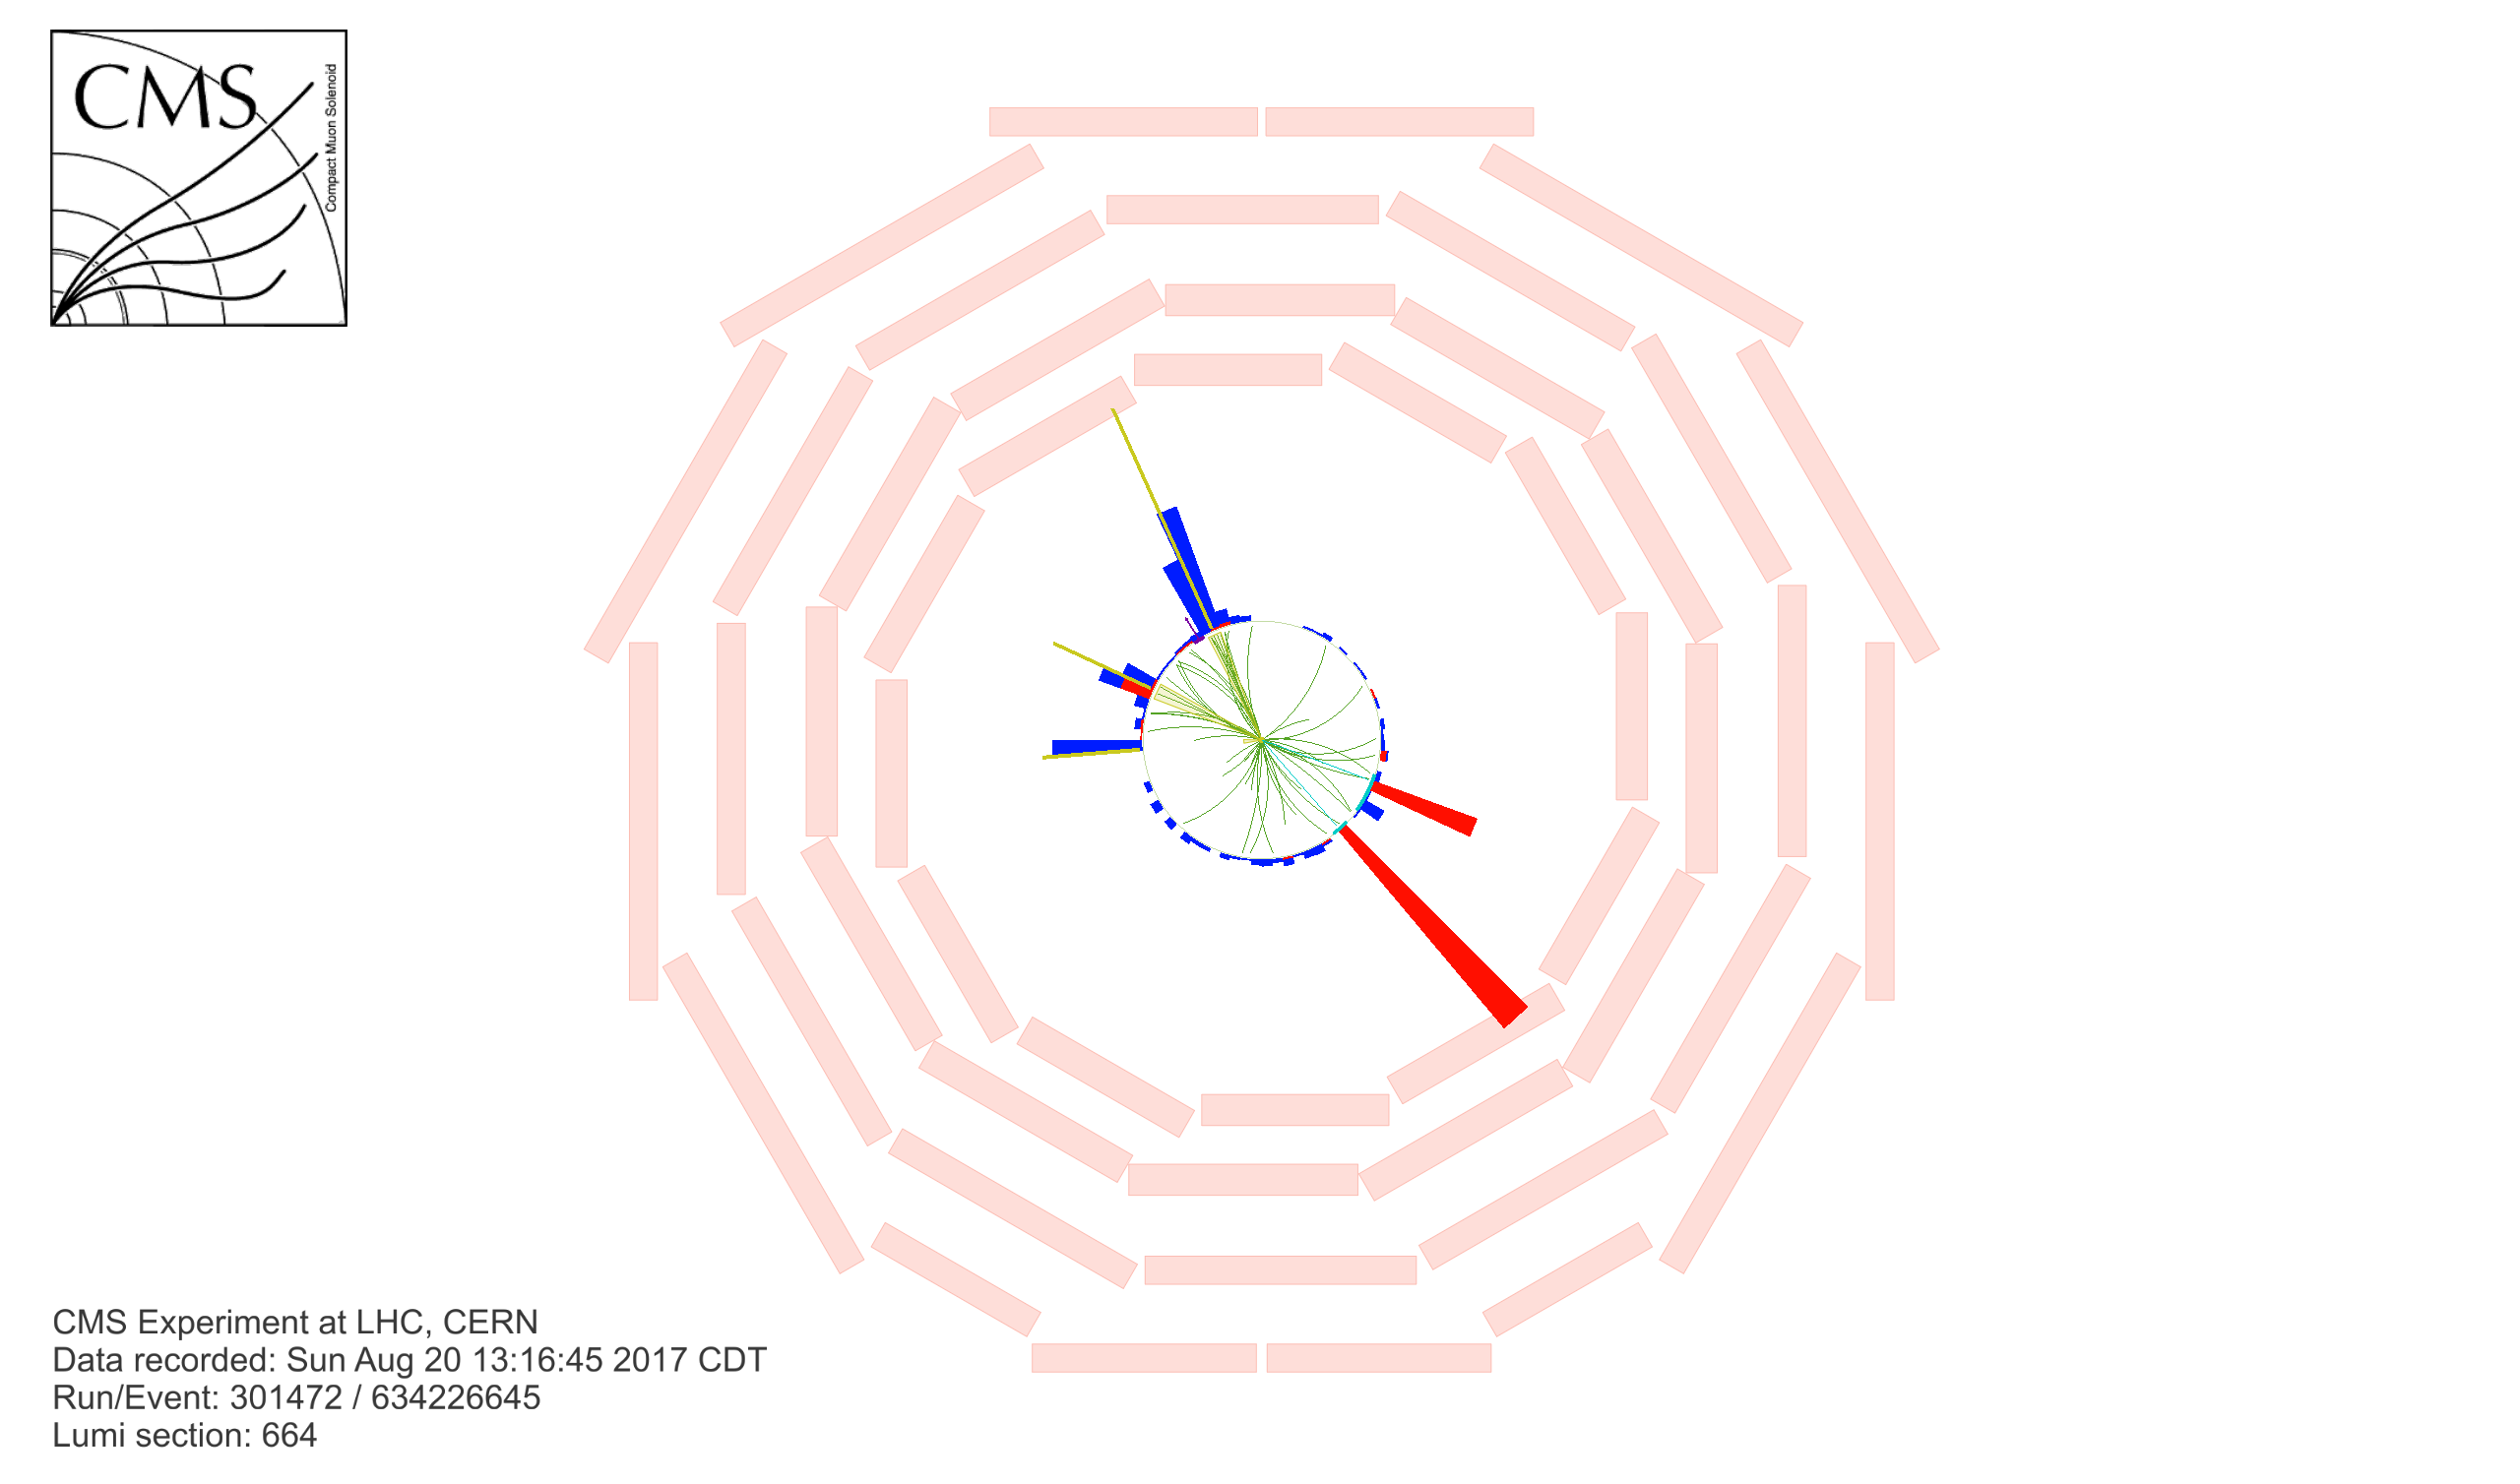
\includegraphics[width=0.5\linewidth]{images/Zee_rhophi_w}}
    \subfigure [] {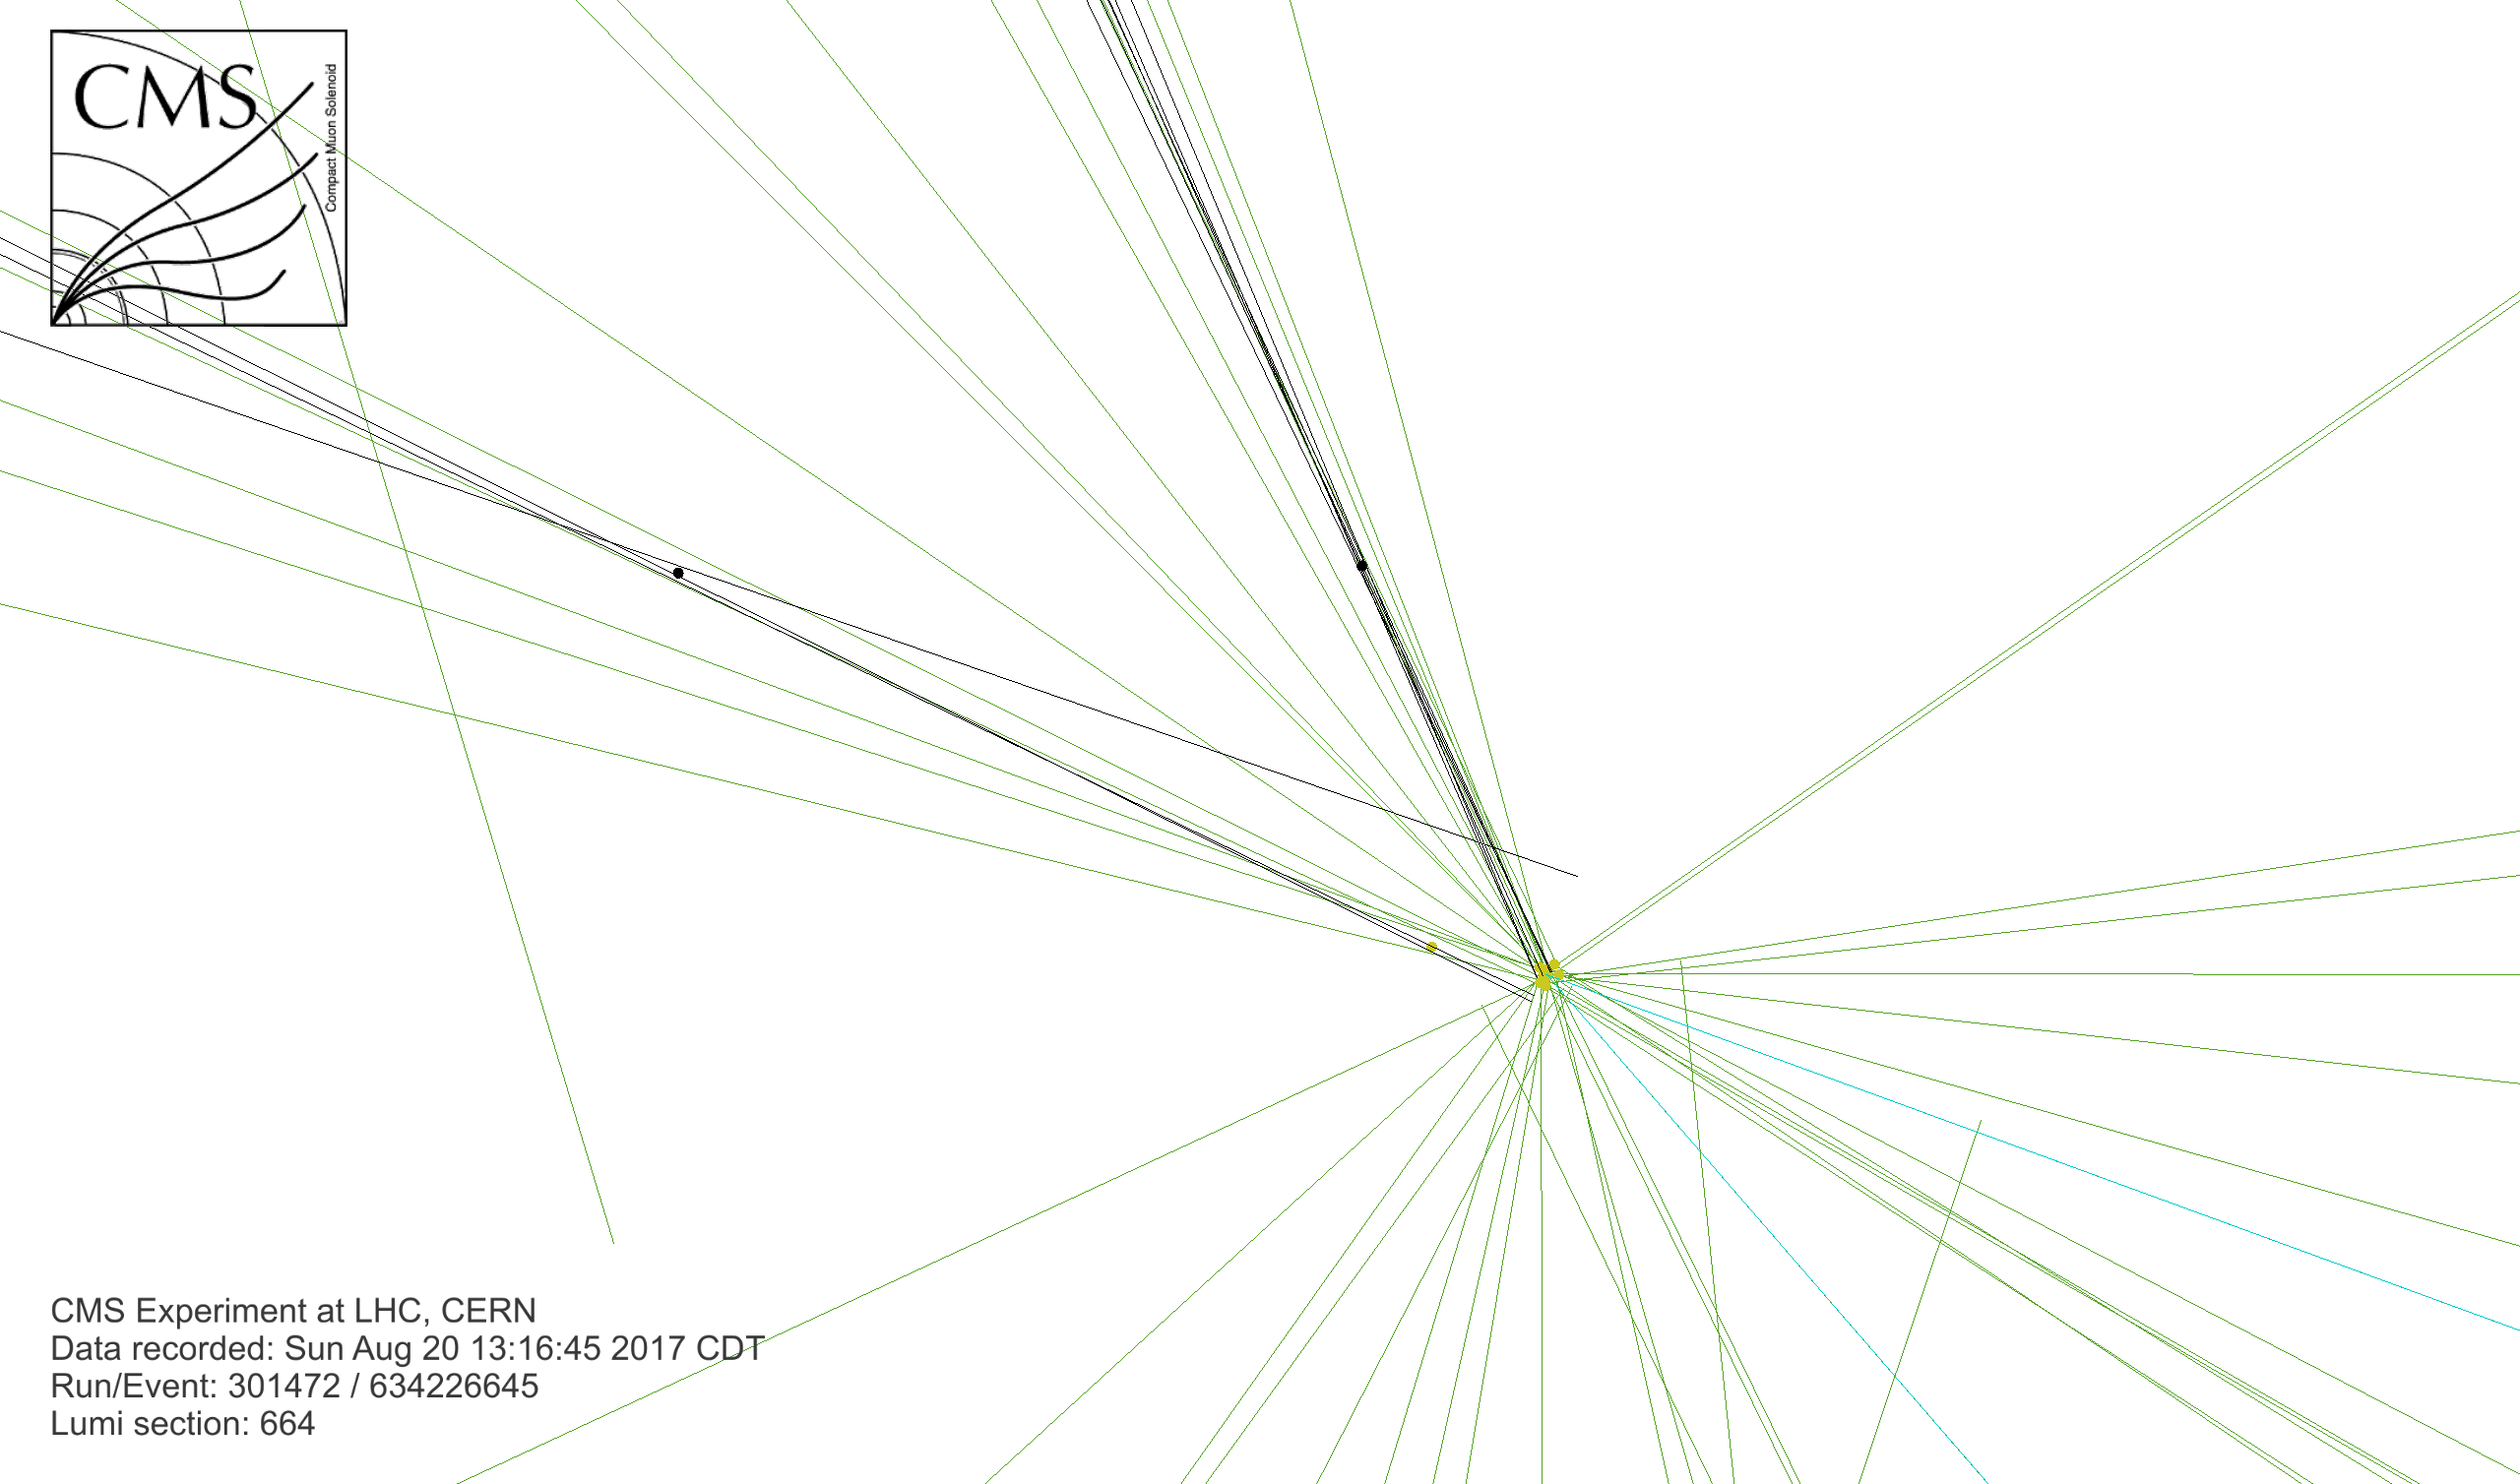
\includegraphics[width=0.5\linewidth]{images/ZeeSV_rhophi_w}}
  }
  \caption[Event Display for \ZeeHbb\ Candidate]{The event display for a candidate \ZeeHbb\ event A) projected onto the \textit{xz}-plane; B) projected onto the \textit{xy}-plane; and C) projected onto the \textit{xy}-plane and zoomed onto the interaction point. The cyan tracks leading to red calorimeter towers represent the electrons from the leptonic decay of the \bosZ\ boson, while the two yellow cones with their blue and red calorimeter towers represent the two \qrkb-jets from the decay of the Higgs boson. The secondary vertices of the \qrkb-jets and their associated tracks (black) are visible in C. The low missing transverse momentum close in azimuthal angle to one of the \qrkb-jets is suggestive of jet energy mismeasurement. This may be related to the blue calorimeter tower without obvious associated tracks, which may have resulted from the decay of a neutral hadron.}
  \label{fig:evt_disp_Zee}
\end{figure}

\begin{figure}[htbp]
  \centering
  \mbox{
    \subfigure [] {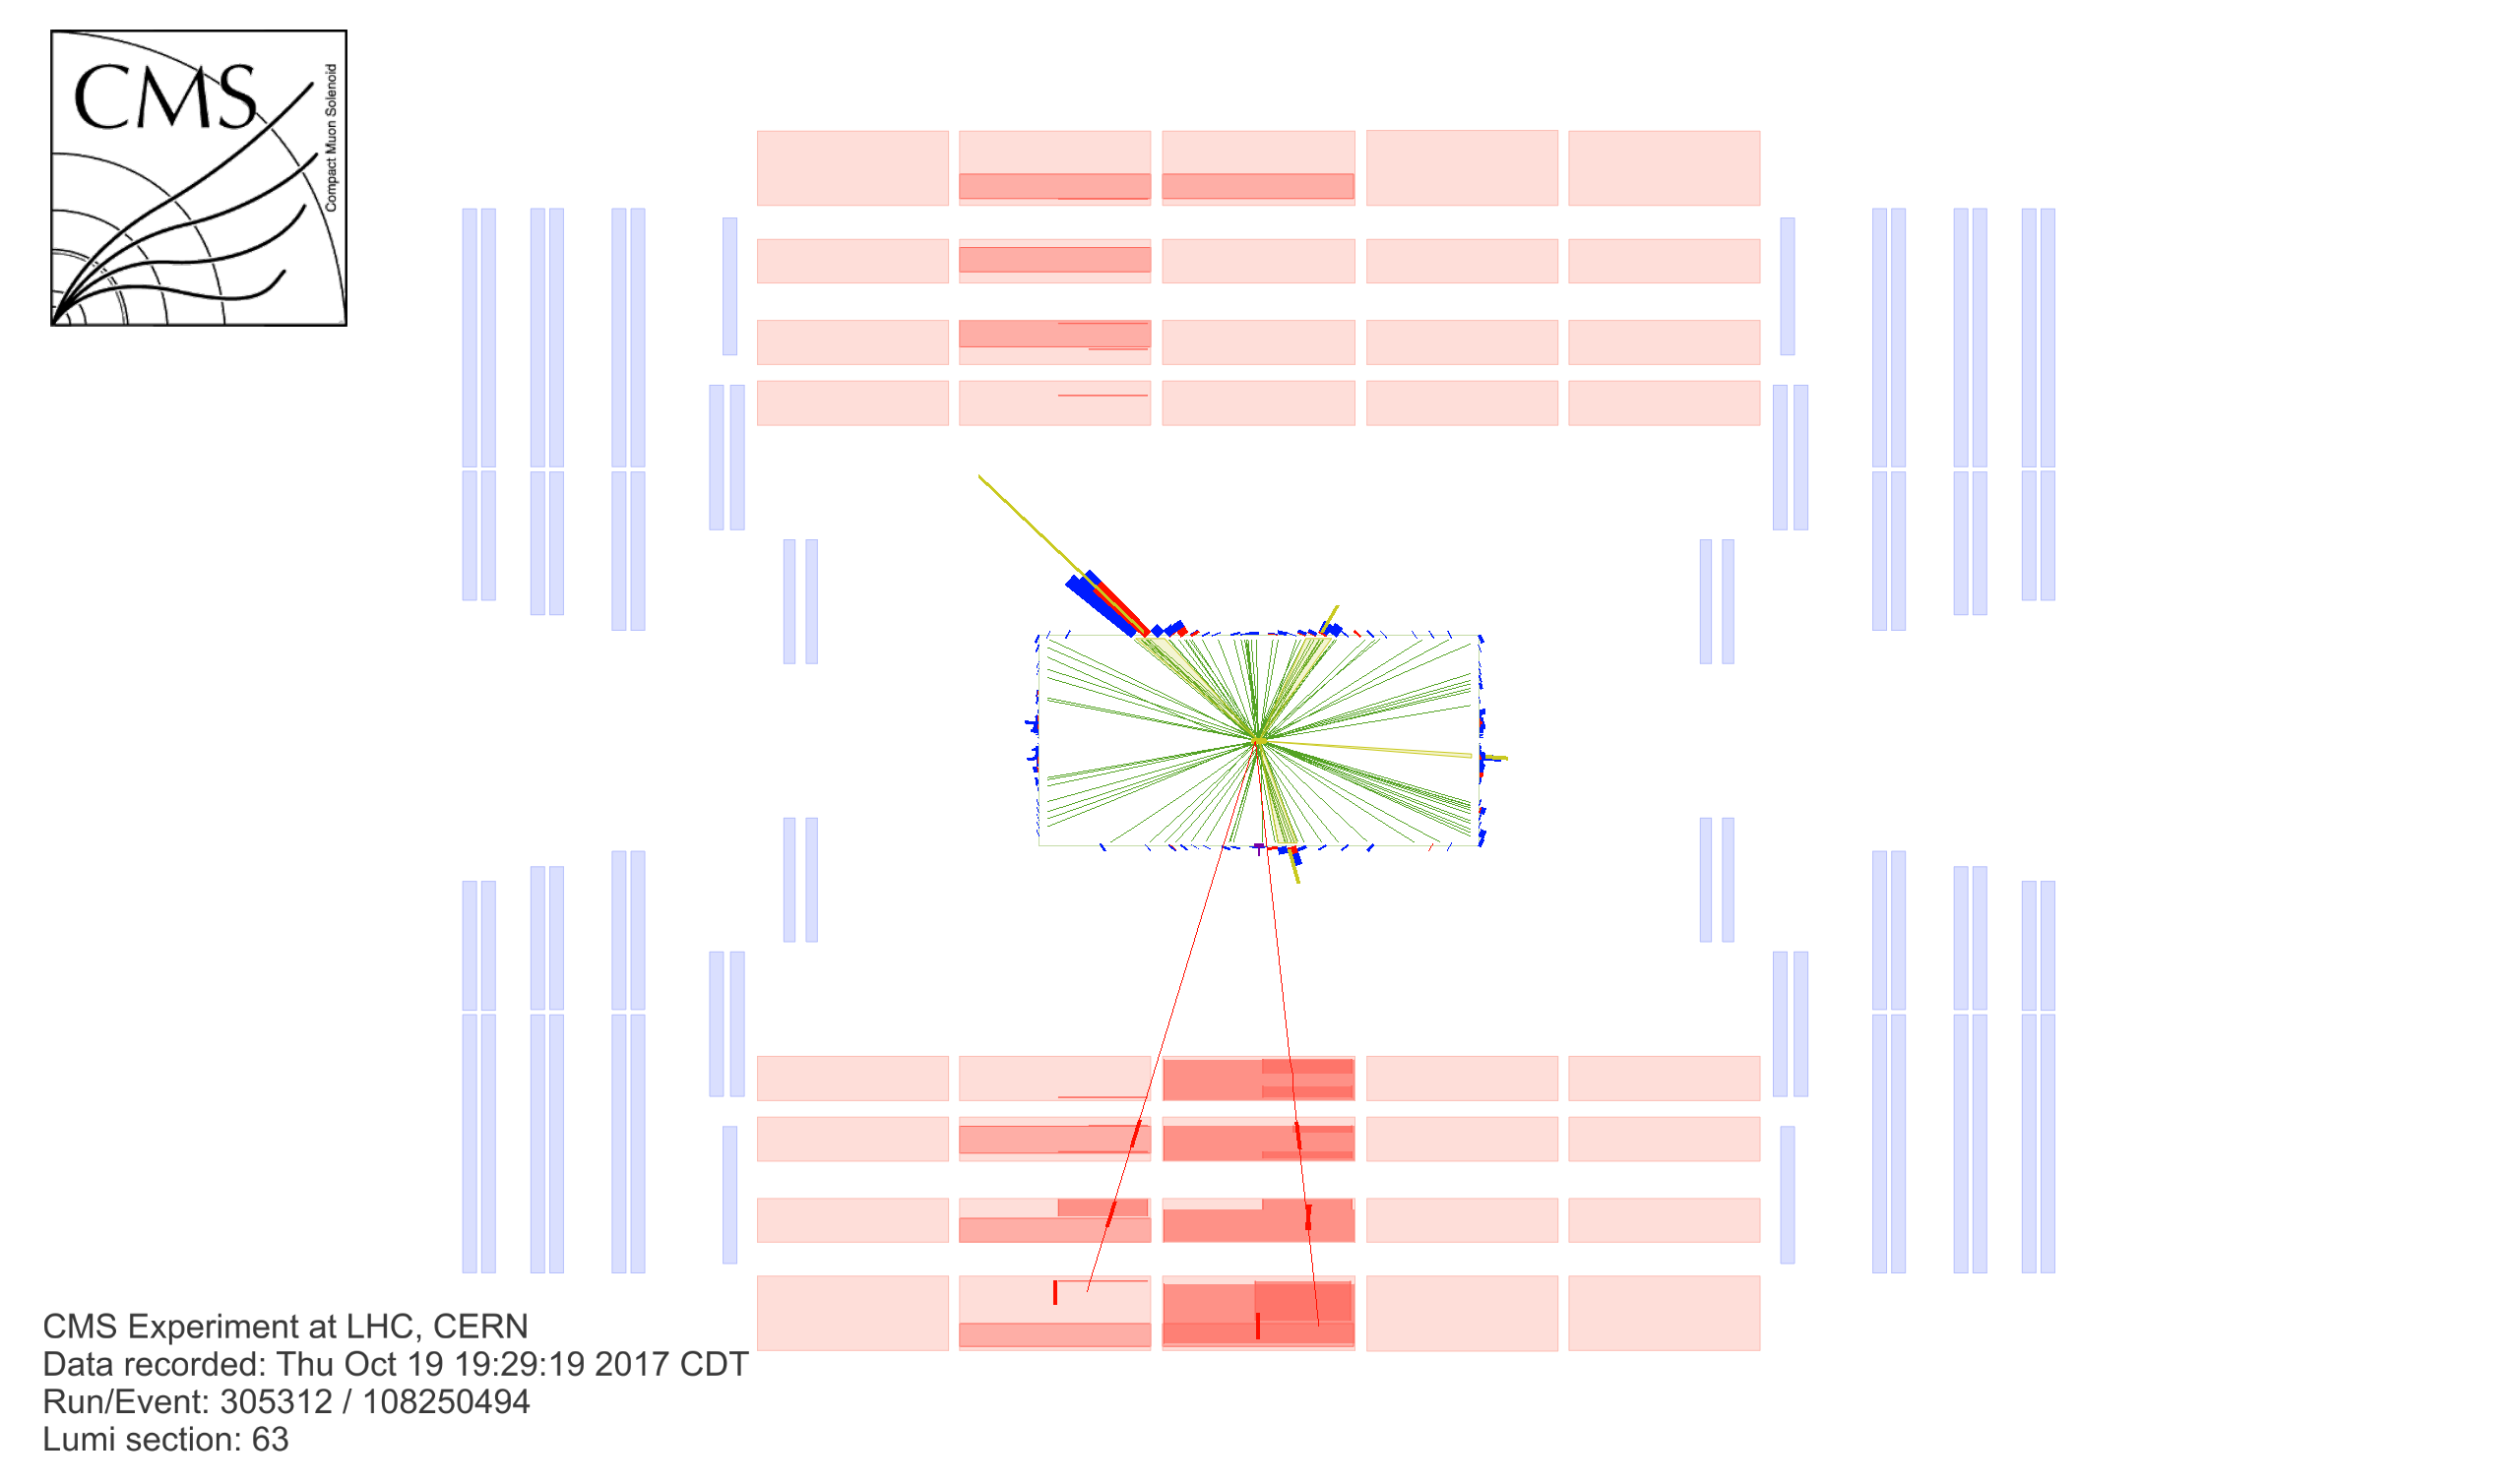
\includegraphics[width=\linewidth]{images/Zmm_rhoz_w}}
  }
  \mbox{
    \subfigure [] {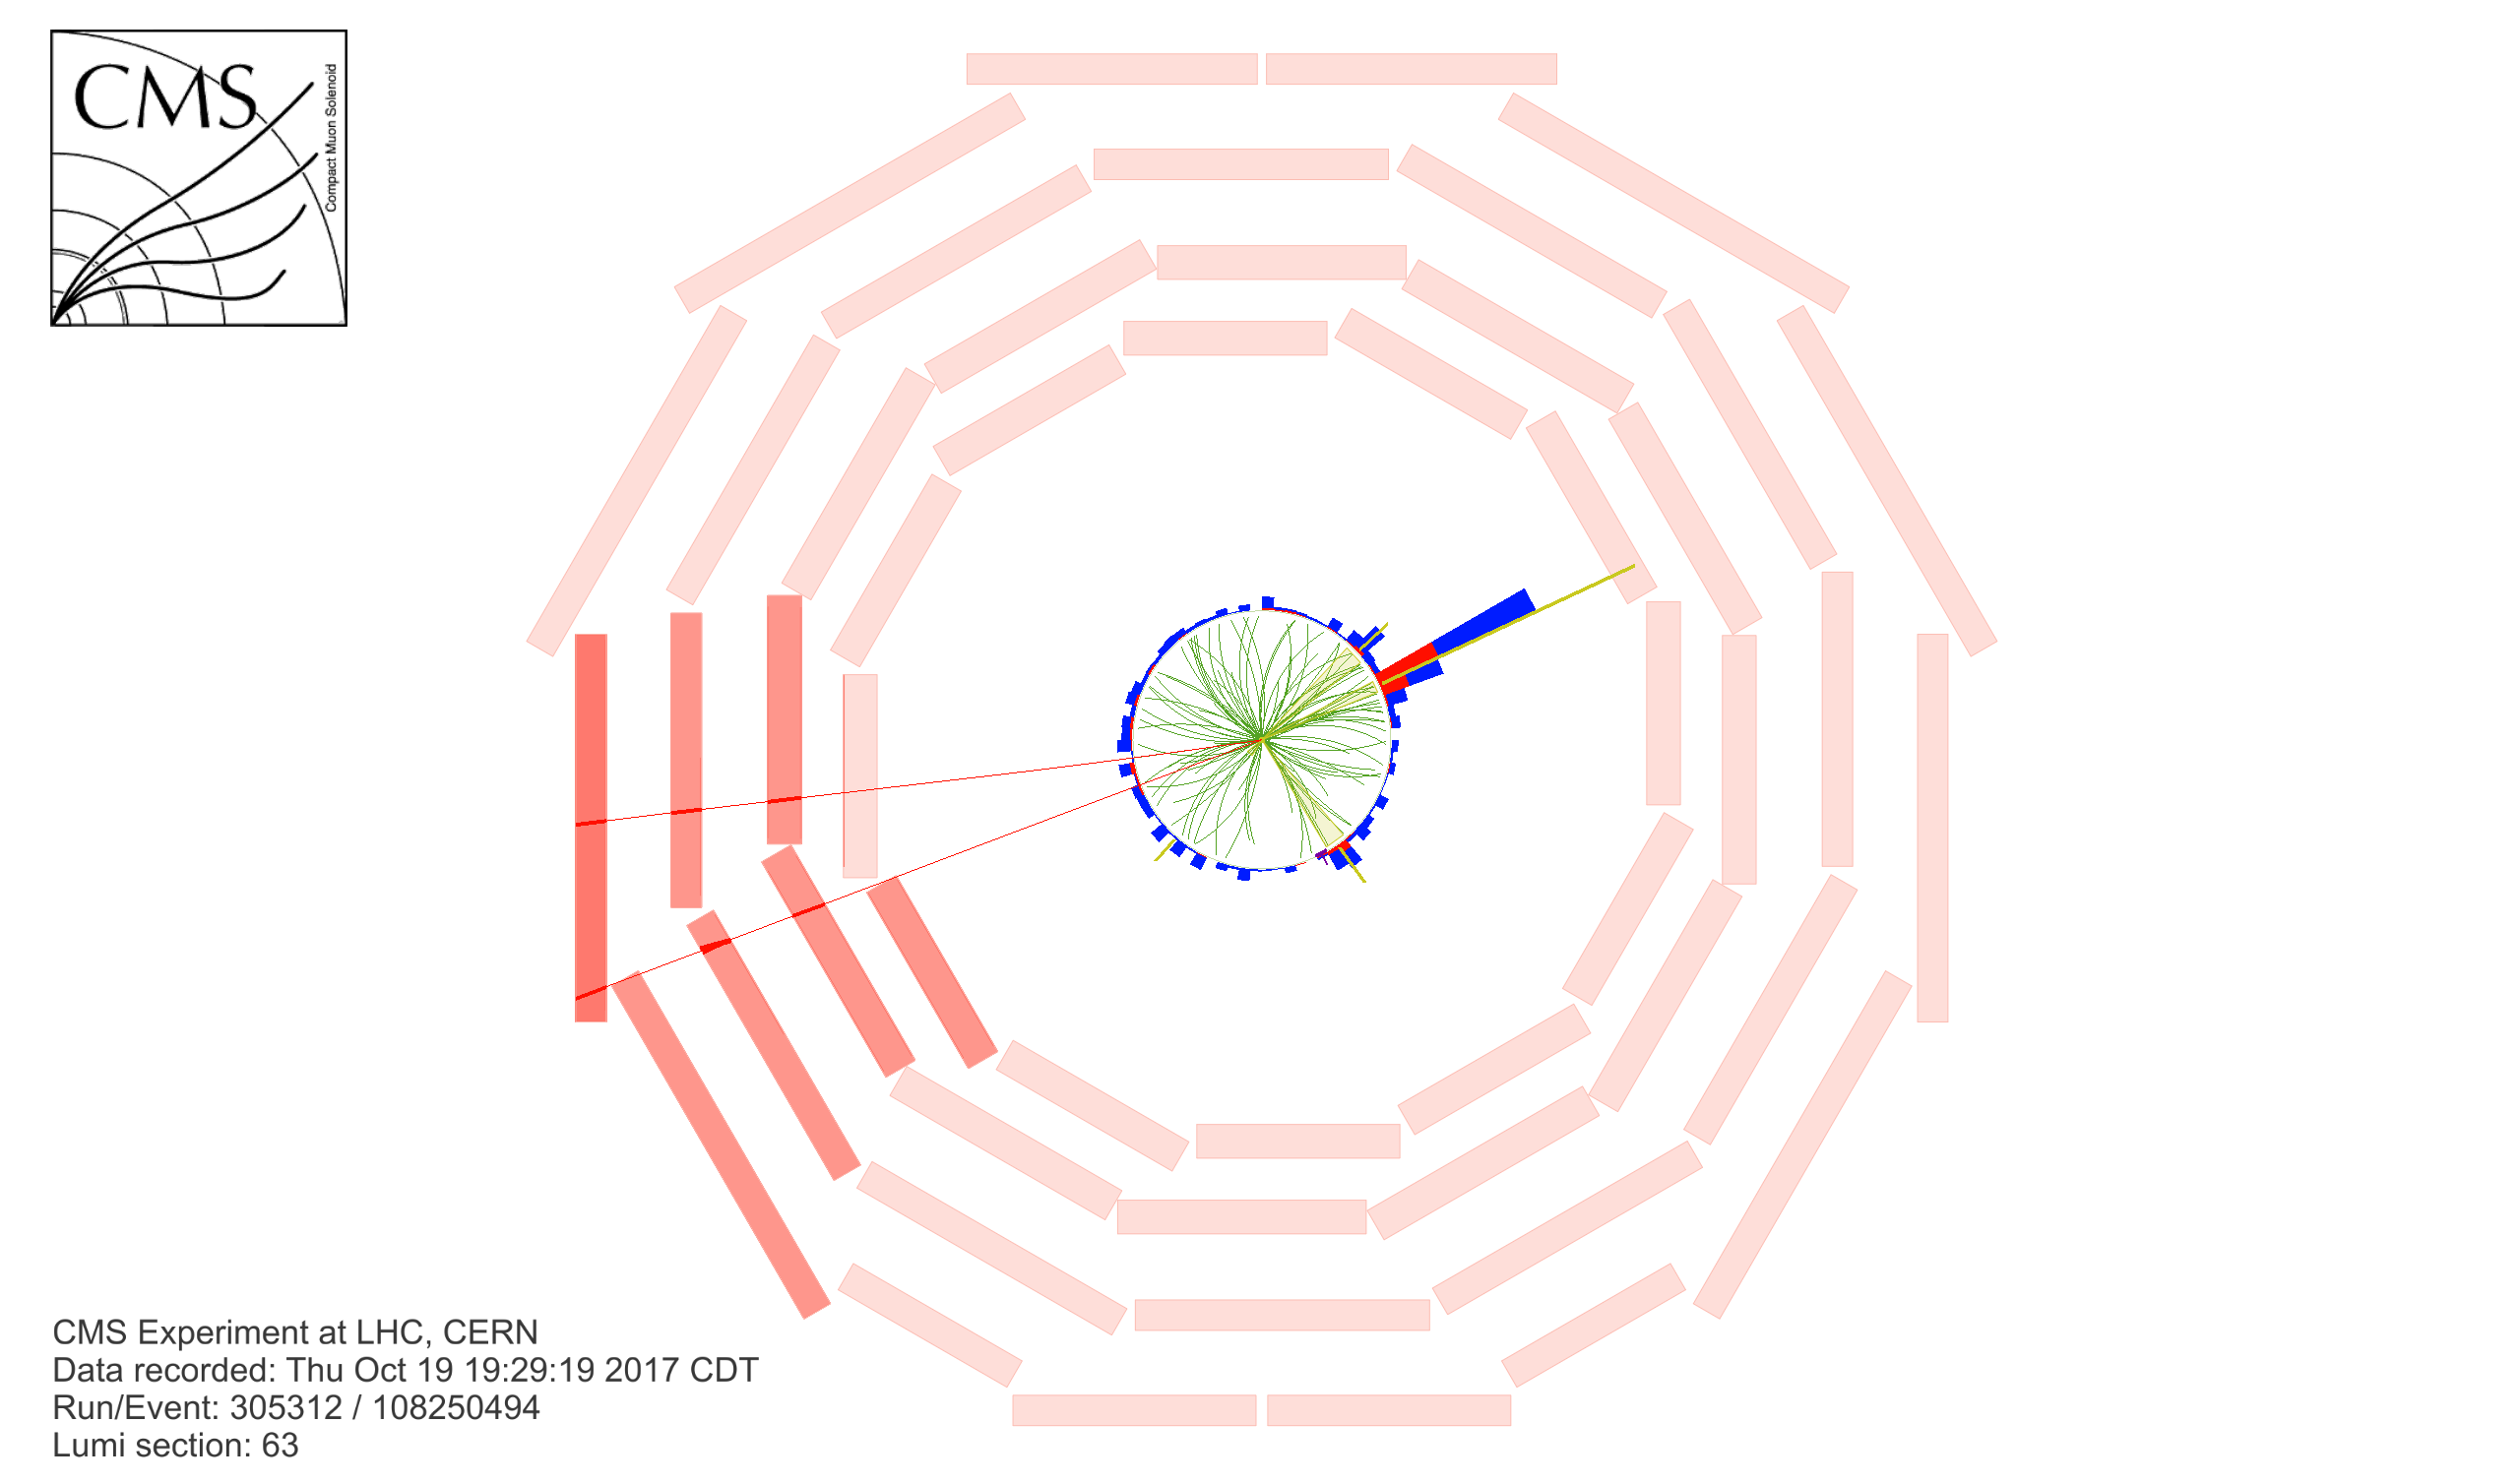
\includegraphics[width=0.5\linewidth]{images/Zmm_rhophi_w}}
    \subfigure [] {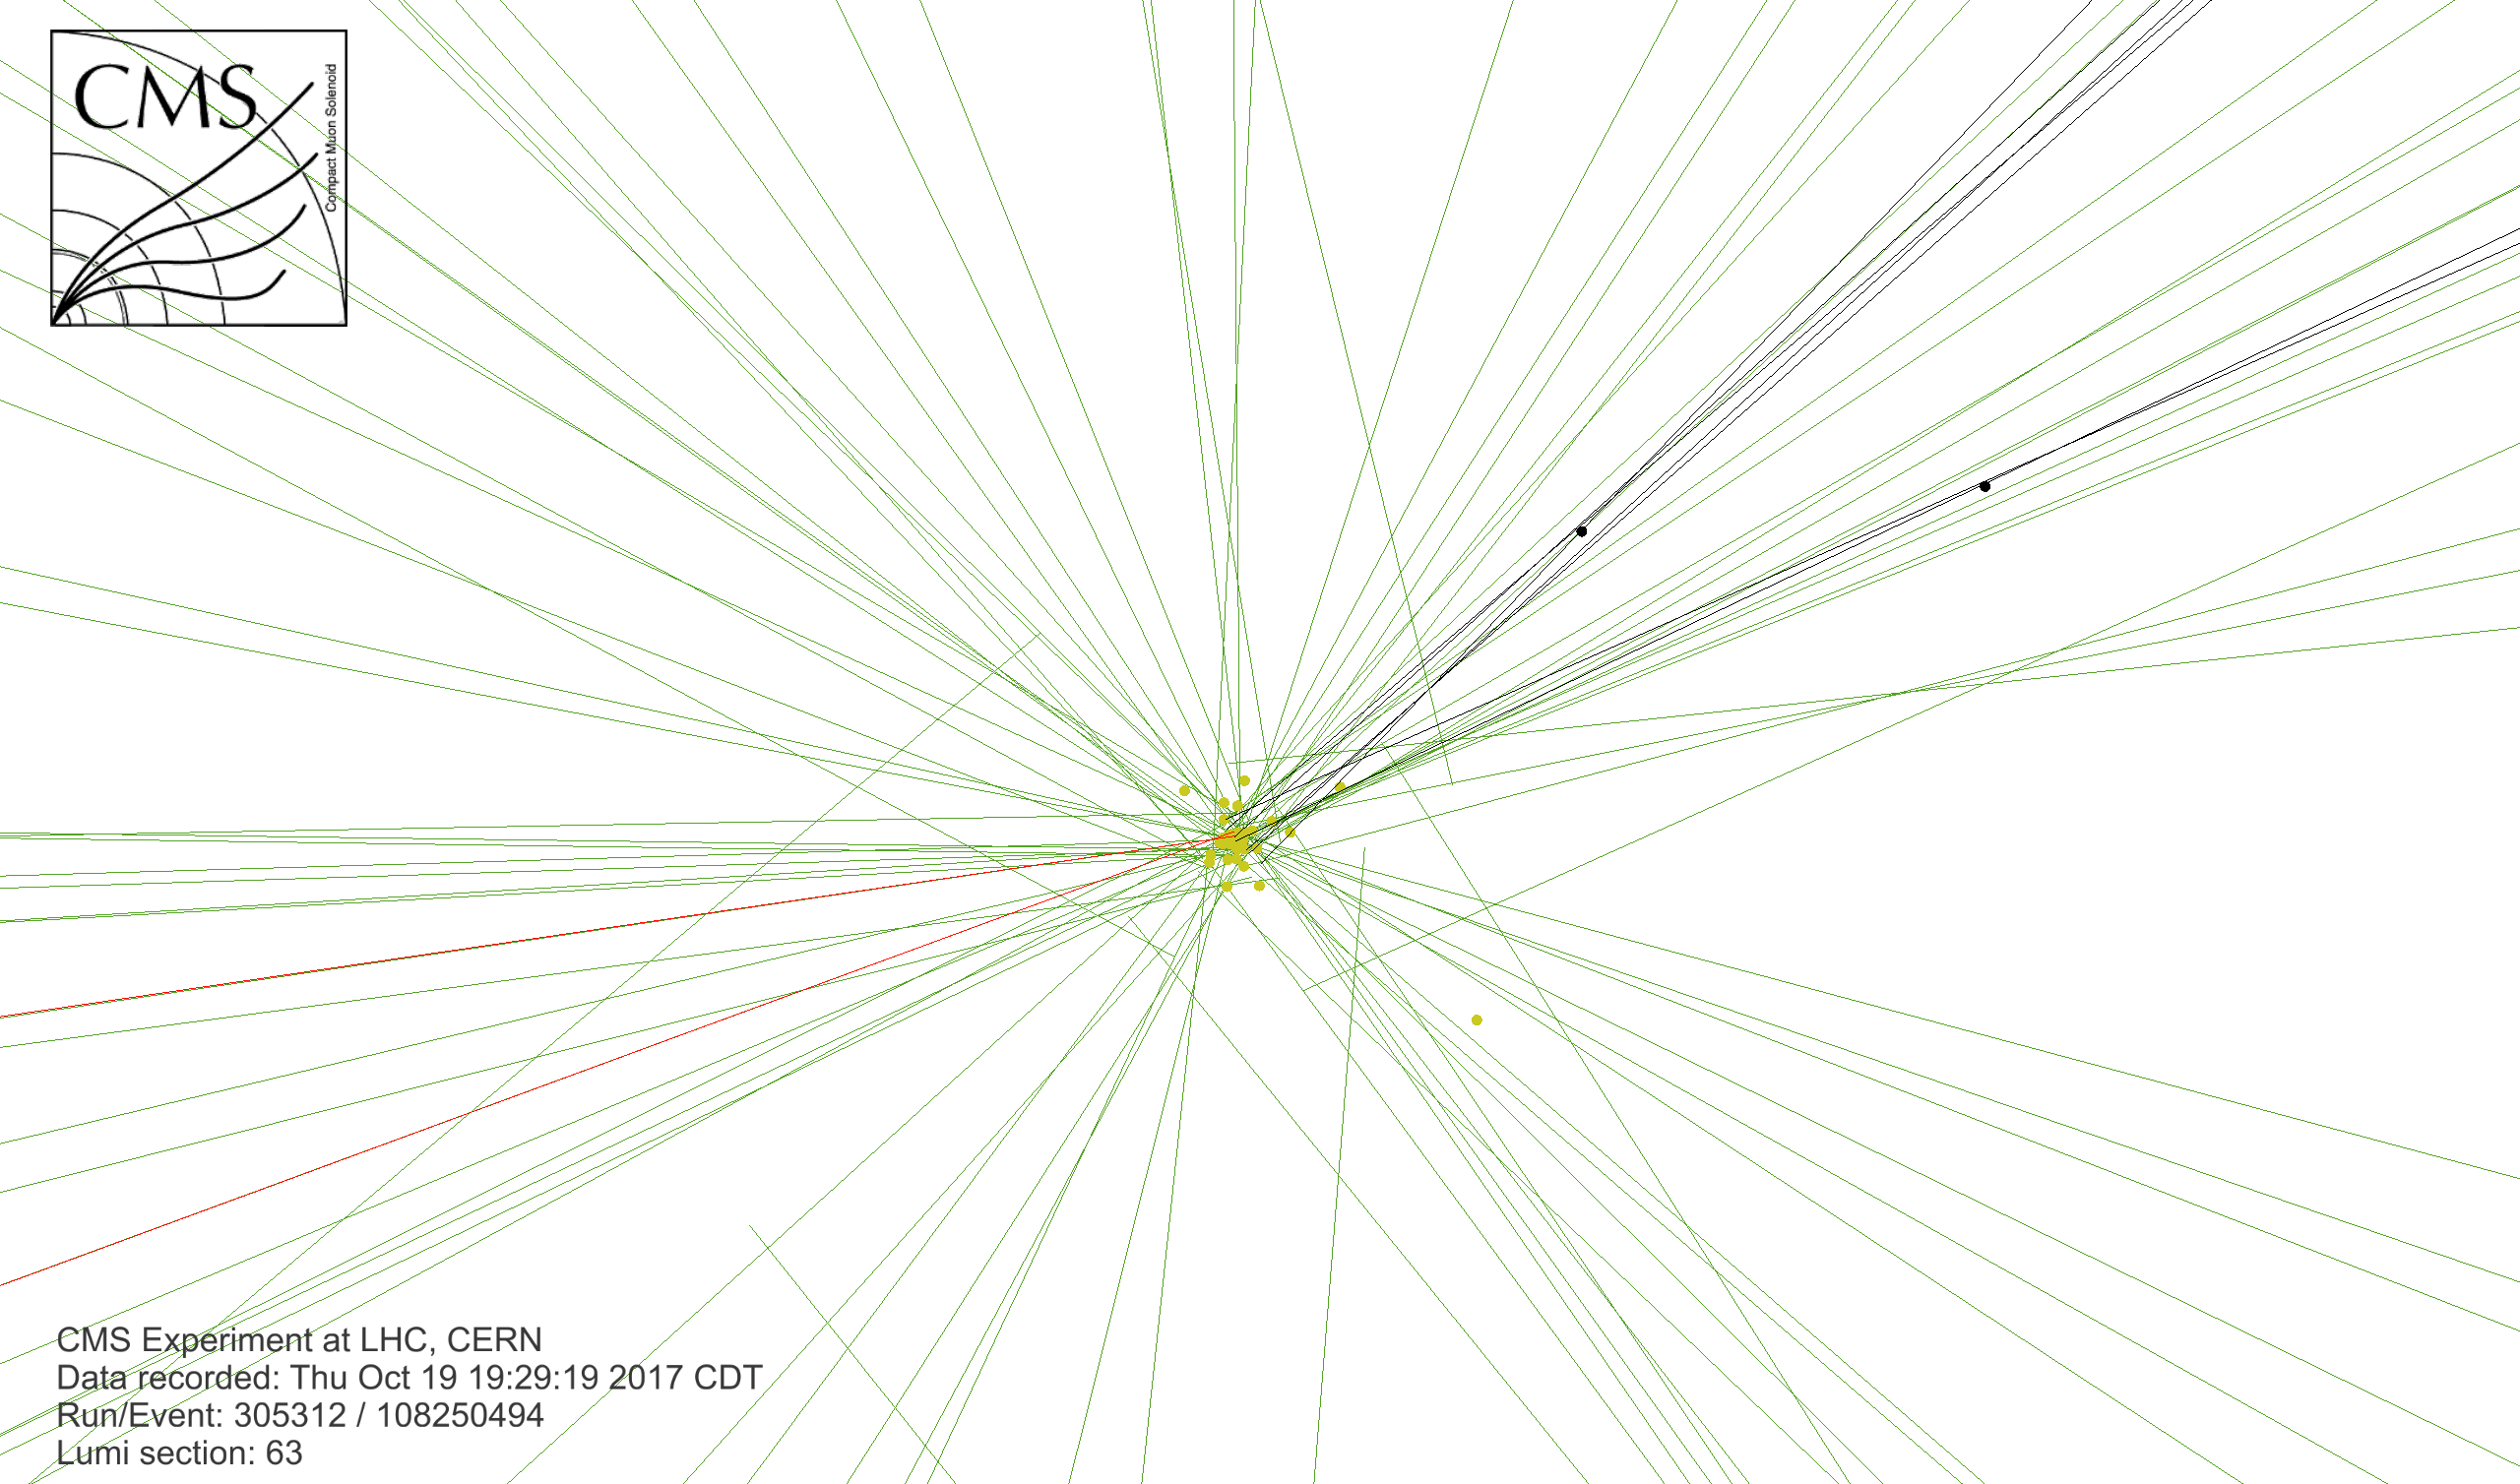
\includegraphics[width=0.5\linewidth]{images/ZmmSV_rhophi_w}}
  }
  \caption[Event Display for \ZmmHbb\ Candidate]{The event display for a candidate \ZmmHbb\ event A) projected onto the \textit{xz}-plane; B) projected onto the \textit{xy}-plane; and C) projected onto the \textit{xy}-plane and zoomed onto the interaction point. The red tracks represent the muons from the leptonic decay of the \bosZ\ boson, while the two yellow cones with their blue and red calorimeter towers located opposite to the red tracks represent the two \qrkb-jets from the decay of the Higgs boson. The secondary vertices of the \qrkb-jets and their associated tracks (black) are visible in C. The two other yellow cones could represent jets caused by initial or final state radiation, neither of which were \qrkb-tagged.}
  \label{fig:evt_disp_Zmm}
\end{figure}

